\section{Postage stamps}\label{sec:postage-stamps}

A postage stamp is a verifiable proof of payment associated with a chunk witnessed by the signature of its owner. On the one hand, postage stamps prevent frivolous uploads by imposing an advance cost. On the other hand, by ascribing a quantity of BZZ, they signal a chunk's relative importance which storer nodes can then use to rank chunks when selecting which ones to retain and serve, and which ones to garbage collect in the event of capacity shortage.

In this section we first introduce the concept of postage batch enabling the bulk purchase of stamps (\ref{sec:purchasing-upload}). In \ref{sec:limited-issuance}, we explain how limited issuance is represented and enforced. In \ref{sec:reserve}, we introduce the notion of reserve and detail the rules governing how storer nodes keep it maximally utilised. We conclude in \ref{sec:depths} with exploring the relationship between reserved capacity, effective demand and the number of nodes and their impact on the data availability.

\subsection{Purchasing upload capacity}\label{sec:purchasing-upload}

% \subsubsection{Postage batches and the postage smart contract}

Uploaders purchase postage stamps in bulk in the form of a \gloss{postage batch} from the postage smart contract on the Ethereum blockchain. Postage batches are created by this contract when a transaction is sent to its batch creation endpoint, together with an amount of BZZ tokens and transaction data specifying some parameters. As the transaction executes, a new batch entry is registered in the postage contract with the following pieces of information:

\begin{itemize}[noitemsep]
\item[--] \emph{batch identifier} -- A random ID that is generated to provide reference for this batch.
\item[--] \emph{batch depth} -- Base 2 logarithm of the \gloss{issuance volume}, i.e., number of chunks that can be stamped using this batch. 
\item[--] \emph{owner address} -- The Ethereum address of the owner entitled to issue stamps, as per the transaction data sent along with the creation or the  transaction sender if not specified.
\item[--] \emph{per-chunk balance} -- The total amount sent along with the transaction divided by the issuance volume.
\item[--] \emph{mutability} -- A boolean flag indicating if the storage slots of the batch can be reassigned to another chunk with a stamp if its timestamp is older. 
\item[--] \emph{uniformity depth} -- the base 2 logarithm of the number of equal-size buckets the storage slots are arranged in.
\end{itemize}

The postage contract provides endpoints to users to modify the per-chunk balance of batches, i.e., add funds to extend the validity period of the stamps issued by the batch (\/\emph{top-up}) or add volume to decrease it (\/\emph{dilute}).
Anyone can then choose to top up the balance of a batch at a later date but only the owner can dilute it.%
%
\footnote{As a planned feature, the remaining balance of a batch can be reassigned to a new batch, resulting in the immediate expiry of the original.}


% \subsubsection{Stamp validity}

\begin{figure}[!ht]
  \centering
    
\includegraphics[width=\textwidth]{fig/postage-stamp-structure.pdf}
  \caption[Postage stamp]{Postage stamp is a data structure comprised of the postage contract batch id, storage slot index, timestamp the chunk address and a witness signature attesting to the association of these four. Uploaders and forwarders must attach a valid postage stamp to every chunk uploaded. }
  \label{fig:postage-stamp}
\end{figure}

Owners issue postage stamps in order to attach them to chunks%
% (see definition \ref{def:postage-stamp} in appendix \ref{sec:appendix-disc})%
. A batch has a number of \glossplural{storage slot} effectively arranged over a number of equal sized buckets. Issuing a stamp means to assign a chunk to a storage slot. A stamp is a data structure comprising the following fields (see figure  \ref{fig:postage-stamp}):

\begin{itemize}[noitemsep]
    \item[--] \emph{chunk address} -- The address of the chunk the stamp is attached to. 
    \item[--] \emph{batch identifier} --  The ID referencing the issuing batch (generated at its creation).
    \item[--] \emph{storage slot} -- An bucket index referencing one of the equal sized buckets of the batch and a within-bucket index referencing the storage slot the chunk is assigned to.
    \item[--] \emph{timestamp} -- The time the chunk is stamped. 
    \item[--] \emph{witness} -- The batch owner's signature attesting to link between the storage slot and the chunk.
\end{itemize}

A postage stamp's validity can be checked by verifying that it scores all true on the following five attributes%
% (see definition \ref{def:postage-stamp-validity} in appendix \ref{sec:appendix-disc})%
:

\begin{itemize}[noitemsep]
\item[--] \emph{authentic} -- The batch identifier is registered in the postage contract's storage.
\item[--] \emph{alive} -- The referenced batch has not yet exhausted its balance.
\item[--] \emph{authorised} -- The postage stamp is signed by the address specified as the owner of the batch. 
\item[--] \emph{available} -- The referenced storage slot is within range given the batch depth, and, in the case of an immutable batch, has no duplicates.
\item[--] \emph{aligned} -- The referenced storage slot has the bucket specified and it aligns with the chunk address stamped.
\end{itemize}

All this can be easily checked by nodes in the swarm only using information available on the public blockchain (read-only endpoints of the postage contract). When a chunk is uploaded, the validity of attached postage stamp is verified by forwarders along the push-syncing route  (see figure \ref{fig:postage-stamps}).


\begin{figure}[!th]
\centering
  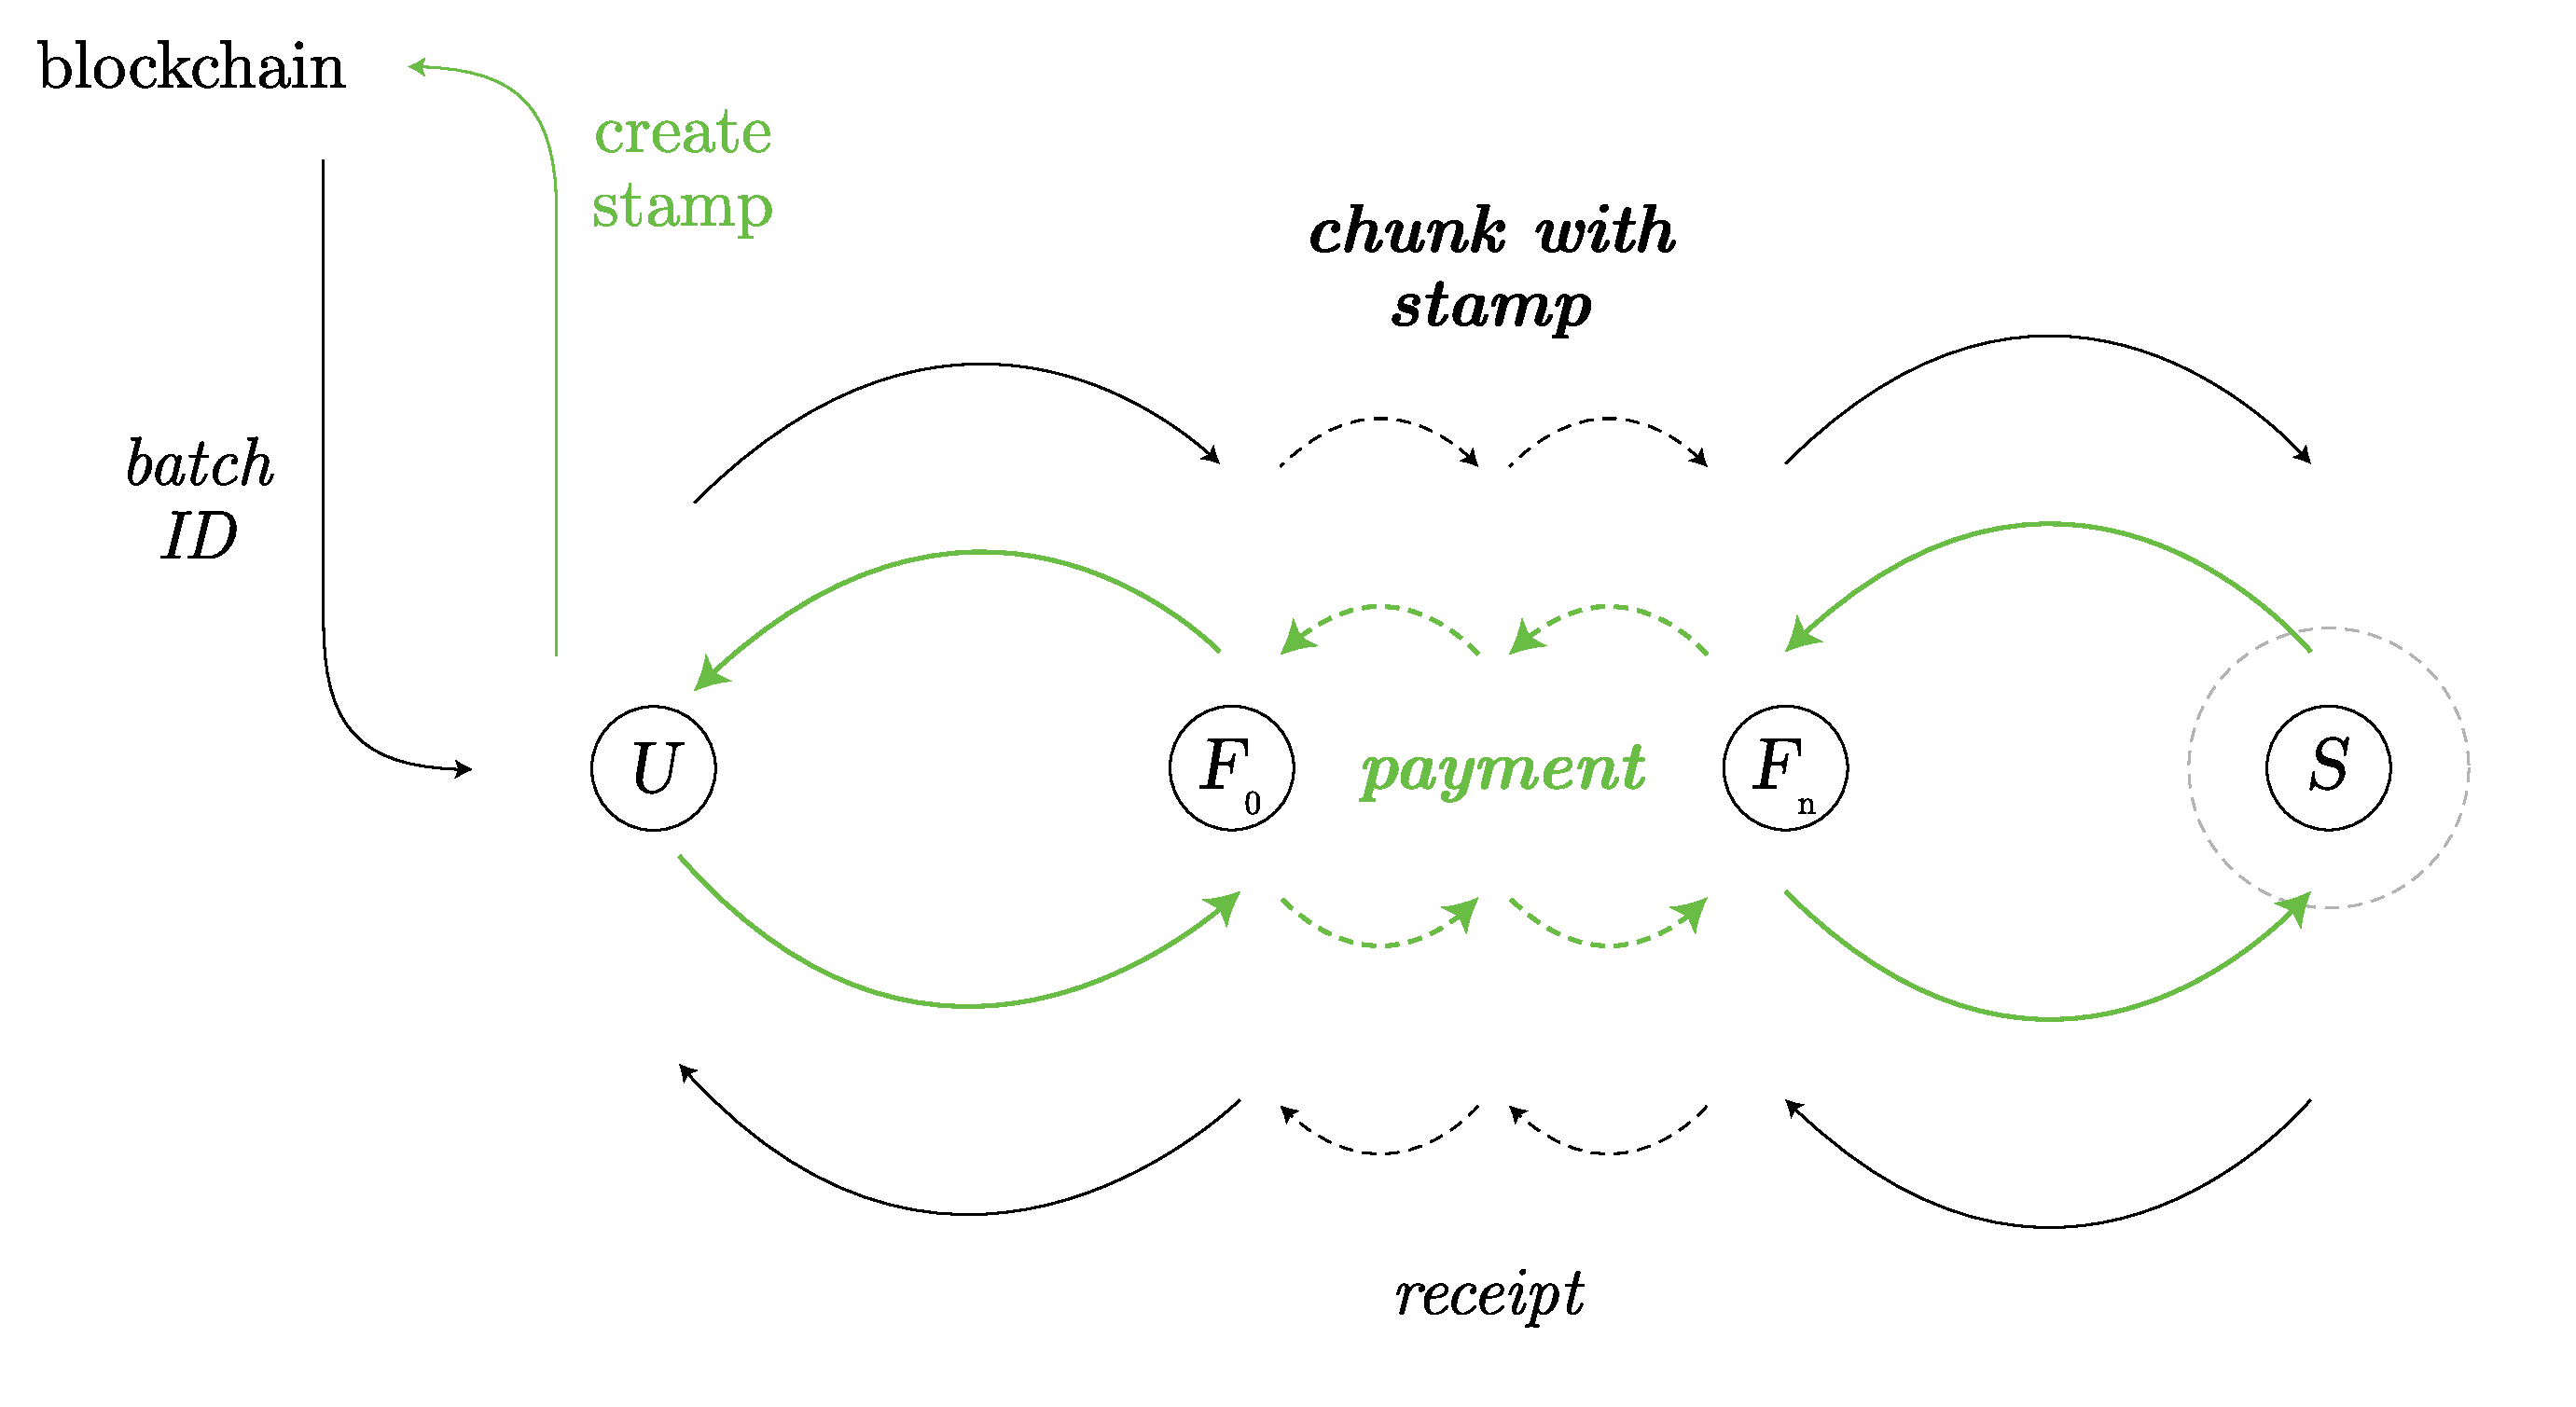
\includegraphics[width=\textwidth]{fig/postage-stamp.pdf}
\caption[Postage stamps]{Postage stamps are purchased in bulk on the blockchain and attached to chunks at upload. They are passed along the push-syncing route together and their validity is checked by forwarders at each hop. }
\label{fig:postage-stamps}
\end{figure}

The normalised per-chunk balance of a batch is calculated as the batch inpayment divided by the batch size in chunk storage slots. The chunk balance is interpreted as an amount pre-committed to be spent on storage. The balance decreases with time as if \emph{storage rent} was paid for each block at the price dictated by the price oracle contract.  

This system allows prepayment for storage without having to speculate on the future price of storage or fluctuations in the currency's exchange rate. At the cost of decreased certainty about the expiration date, one gains resilience against price volatility. On top of this, uploaders can enjoy the luxury of non-engagement by tying up more of the batch balance; while it serves as collateral against price increase, if that does not happen the funds can still be used up (for storing).


\subsection{Limited issuance}\label{sec:limited-issuance}

% \subsubsection{Issuing postage stamps}

Purchasing a postage batch effectively entitles the owner to issue a fixed amount of postage stamps against the batch ID called the \gloss{issuance volume} or \gloss{batch size}. It is restricted to the powers of 2 and is specified using the base 2 logarithm of the amount which is called \gloss{batch depth}. Storage slots of a batch are arranged in a number of buckets and are indexed within the bucket. The number of buckets is restricted to the powers of 2 and is specified using its base 2 logarithm called \gloss{uniformity depth}. The size limitation of a batch with batch depth $d$ and uniformity depth $u$ is equivalent to the conditions that 1) the bucket index ranges from 0 to $2^u-1$, 2) the within-bucket index ranges  from 0 to $2^{d-u}-1$ and 3) there are no duplicate indexes.  

While 1) and 2) is easily verifiable by any third party, 3) is not.
In order for index collisions to be detectable by individual storer nodes, uniformity depth must be large enough to fall within nodes' area of responsibility.
As long as this is maintained, all chunks in the same bucket are guaranteed to land in the same neighbourhood, and, as a result, duplicate assignments can be locally detected by nodes (see figure \ref{fig:over-issuance}).

In order to keep their stamps collision-free, uploaders need to maintain counters for how many stamps they have issued for each bucket of a batch and must not issue more than the allowed bucket size. 

\begin{figure}[!ht]
  \centering
    
\includegraphics[width=1\textwidth]{fig/batch-structure.pdf}
  \caption[Batch structure, uniformity and over-issuance]{Batches come with $2^u$ equal-sized buckets ($u$ is uniformity depth, orange circle) each containing an equal number of storage slots ($2^{d-u}$) adding up to batch capacity of $2^d$ chunks ($d$ is batch depth, red circle). Storage slots are indexed and the index is associated with a chunk via the stamp signature. Postage stamp over-issuance is detected locally by storer nodes as long as the buckets are deeper than their storage depth (green circle), as in the diagram on the left. In this case they will receive all the chunks that are correctly assigned to the relevant bucket (orange radii) and correctly identify collisions (red radii) by forbidding indexes that are either out of range ($\geq 2^{d-u}$) or multiply assigned. In contrast, the diagram on the right shows it is not possible for a node with storage depth 4 to identify duplicates for a batch with $u=2$.}
\label{fig:over-issuance}
\end{figure}    



In general, the most efficient utilisation of a batch is by filling each bucket fully. 
%
%
% \footnote{See appendix \ref{sec:batch-utilisation} for a detailed analysis of batch utilisation.
% \subsubsection{Efficiency of batch utilisation}
% }
%       
Continued non-uniformity (i.e., \emph{targeted issuance}) leads to underutilised batches, and therefore a higher unit price for uploading and storing each chunk. This feature has the desired side effect that it imposes an upfront cost to non-uniform uploads: the more concentrated the distribution of chunks of an upload, the more storage slots of the postage batch remain unused. In this way, we ensure that targeted denial-of-service attacks against a neighbourhood (i.e., uploading a disproportionate number of chunks in a particular address range) is costly since the \emph{inert cost} (due to the degree of under-utilisation of the batch) is exponential in the depth of the skew.

Beyond DoS protection, postage stamps can serve as a \emph{fiduciary signal} indicating how much it is worth for a user to persist a chunk in Swarm. In particular, the per-chunk balance of batches can provide the differential a priori bias determining which chunks should be protected from garbage collection in the absence of evidence to predict their profitability from swap. 



\subsection{Rules of the reserve}\label{sec:reserve}

% \subsubsection{Batch balance, rent and expiry}\label{sec:rent-expiry}

The \gloss{reserve} is a fixed size of storage space dedicated to storing the chunks in the node's \gloss{area of responsibility}. Chunks in the reserve are the chunks that are protected against garbage collection with valid postage stamps. When batches expire, i.e., their balance is completely depleted, the chunks they stamped are no longer protected from eviction. Their eviction from the reserve frees up some space that can accommodate new or farther chunks belonging to valid batches.


From the point of view of incentives, chunks which are of the same proximity order and the same batch are equivalent. When it comes to eviction due to batch expiry, these equivalence classes, called \gloss{batch bins} are handled as one unit: the chunks in a batch bin are evicted from the reserve and inserted to the cache in one atomic operation. 

Assuming a global oracle for the unit price of rent and a fixed reserve capacity  prescribed for nodes, the content of the reserve is coordinated with  a set of constraints on batch bins called the \gloss{rules of the reserve}:
\begin{itemize}[noitemsep]
    \item[--] if a batch bin of a certain PO is reserved then the batch bins are reserved also for all closer bins (higher PO). 
    \item[--] if a batch bin is reserved at a certain proximity order (PO), then all the batch bins at the same PO belonging to batches with a greater per-chunk balance are also reserved. 
    \item[--] the reserve should not exceed capacity.
    \item[--] the reserve is maximally utilised, i.e, cannot be extended and have 1-3 remain true.
\end{itemize}

The first rule means the reserve is closed upwards for PO, which encodes a global preference for  chunks closer to the node's address. This is incentivised by routing: keeping the closest chunks, a node will maximise the number of receipts it can issue and the number of retrieve requests it can respond to and at the same time provides the widest coverage within the neighbourhood even after the neighbourhood is no longer supporting the desired redundancy.

The second rule expresses the constraint that the reserve for a PO is upward closed for per-chunk balance, which encodes a secondary preference among chunks of the same proximity for those stamped using a batch with higher per-chunk balance. This is incentivised by the differential absolute profit chunks promise: due to the  constraint that balances are not revocable, chunks with higher balance expire later and therefore contribute more to storers' absolute profit than those expiring earlier despite the same rent paid during their period of validity.%
%
\footnote{Note that even if there was no scheme for redistributing postage revenue and the inpayments are frozen/burnt, this strategy is still mildly incentivised in as much as it is aligned with token-holders interest: batches with higher balance exert more deflationary force on the token (per chunk, i.e, the unit of invested resource) by keeping their balance frozen which is expected to realise in a proportional price increase.}


\begin{figure}[!ht]
  \centering
    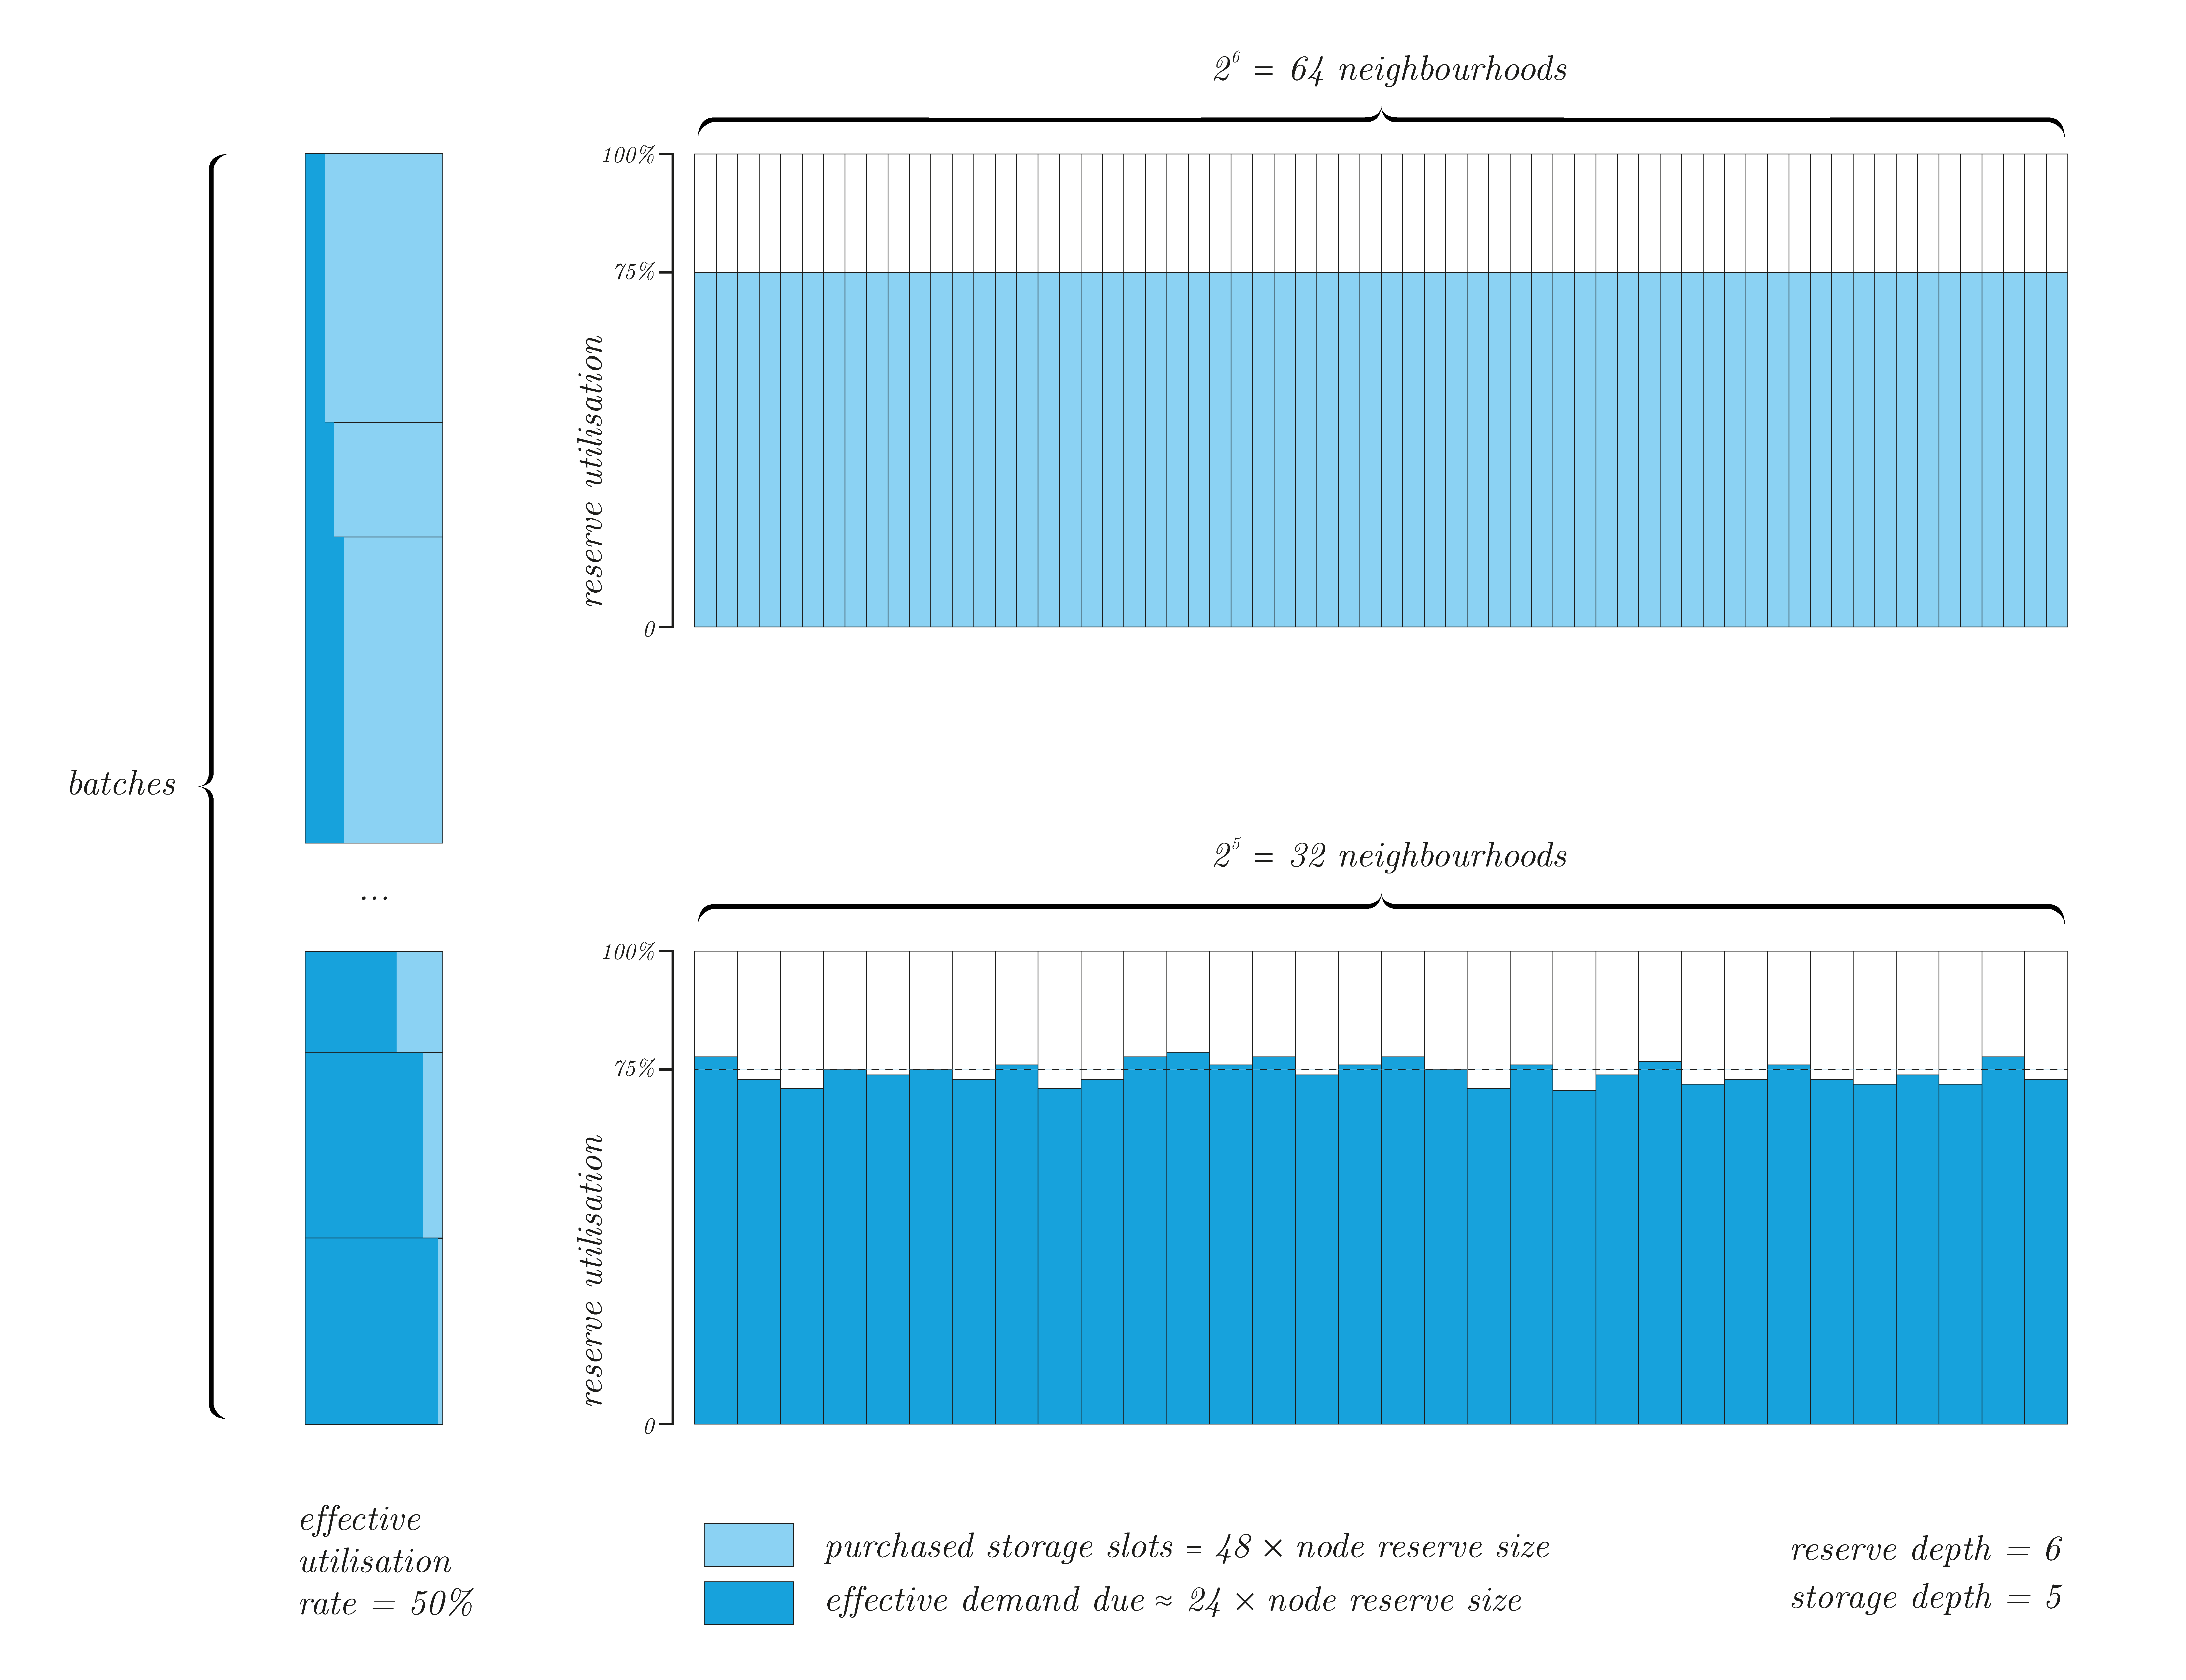
\includegraphics[width=.9\textwidth]{fig/supply-demand.pdf}
  \caption[Reserve capacity]{Potential demand for chunk storage is expressed by the total size of all batches with non-zero balance on the blockchain (left). The lower bound on neighbourhood depth to store this capacity is the reserve depth (top right). Storage depth marks the effective volume of chunks uploaded and stored in a neighbourhood's reserve (bottom right). The difference between them is a result of partial batch utilisation. The uniformity of the volume of chunks across neighbourhoods is incentivised by the efficient utilisation of postage batches.}
\label{fig:reserve-capacity}
\end{figure}    

When a new chunk arrives in swarm through pull-sync, push-sync or upload, the validity  of the attached  postage stamp is verified. If the PO of the chunk is lower than the batch depth, the node inserts the chunk into the  garbage collection index, otherwise it is by definition in the reserve. 
If the reserve size is above capacity, a number of batch bins are identified so that their total size covers the excess so that after these batch bins are \emph{evicted} from the reserve, the reserve size will be within capacity. 


\subsection{Reserve depth, storage depth, neighbourhood depth}\label{sec:depths}



\subsubsection{Reserve depth}

The potential demand for chunks to be stored in the DISC is quantified by the total storage slots of valid batches. This is calculated as the sum of the sizes of non-expired batches. Since the batches and their balances are recorded in the postage contract, the reserved DISC size is under consensus.%
%
\footnote{The volume is best explicitly maintained by the contract by adding the size of newly created batches and deduct the sizes of newly expired batches. DISC reserve size is updated each time a batch is created or topped up and expired batches are removed during each redistribution round, executed as part of the process triggered by the claim transaction.}  

The base 2 logarithm of the DISC reserve size rounded up to the nearest integer is called the \gloss{reserve depth}. The reserve depth is the shallowest PO such that disjoint neighbourhoods of this depth are collectively able to accommodate the volume of data corresponding to the total number of chunks paid for, assuming that nodes in the neighbourhood have a fixed prescribed storage capacity to store their share of the reserve. 

The reserve depth is also the \emph{safe lower bound} for pull-syncing, i.e, the farthest bin a neighbourhood needs to synchronise to guarantee storing the reserve.
Conversely, if any neighbourhood marked by reserve depth has no nodes in it, the swarm is not working correctly, i.e., chunks with valid stamps are not protected from getting lost. See figure \ref{fig:depths}.

\subsubsection{Storage depth}

The \gloss{effective demand} for chunks to be stored in the DISC is the total number of chunks actually uploaded. While each chunk in the reserve has a valid postage batch and therefore is assigned to a storage slot, a postage batch can always have some of its storage slots unassigned. This entails that the number of chunks actually stored in the DISC can in fact be a fraction of the DISC reserve size. 

The effective area of responsibility is  marked by the proximity order of the farthest batch bin of the reserve assuming the node complies with the rules of the reserve. 

A node's \gloss{storage depth} is defined as the shallowest \emph{complete} bin, i.e., the lowest PO that compliant reserves stores all batch bins at. Unless the farthest bin in the node's reserve is complete, the storage depth equals the reserve's edge PO plus one.

The storage depth is the \emph{optimal lower bound} for pull-syncing, i.e, the farthest bin the node needs to synchronise with its neighbours to achieve maximum reserve   utilisation.%
%
\footnote{The nodes will have full connectivity up to the shallowest bin that they are pull syncing. This choice is incentivised by the risk of having two disjoint connected sets of pull-syncing nodes resulting in non-consensual reserve. As a consequence, we can say that storage depth is an upper bound on the depth of full connectivity.}
%
Maximum reserve utilisation should be incentivised as part of the storage incentives. 

% See figure \ref{fig:reserve-depth-vs-storage-depth}.

% \begin{figure}[!ht]
%   \centering
%     % \includegraphics[width=\textwidth]{fig/reserve-depth-vs-storage-depth.pdf}
%   \caption[Reserve depth vs storage depth]{Reserve depth vs storage depth.}
% \label{fig:reserve-depth-vs-storage-depth}
% \end{figure}    




% \subsubsection{Batch utilisation rate}\label{sec:utilisation-rate}

The gap between actual storage depth and the  reserve depth exists because of the bulk purchase of stamps. Since entire batches of stamps reserve storage slots that are assigned to  chunks only at later times when they are actually uploaded, the batch \emph{utilisation rate} can be substantially less than 1%
% (see appendix \ref{sec:batch-utilisation})%
. Storage depth and reserve depth are the same only if all batches are fully utilised. 


\subsubsection{Neighbourhood depth}

Swarm's requirements on local replication is that each neighbourhood designated by the storage depth contains at least four nodes. 
If neighbourhoods were made of one node, then the outage of that one node will make  the chunks in the node's area of responsibility not retrievable.
With two nodes in a neighbourhood, we significantly improve resilience against ad-hoc outages, but because of connectivity latencies a two-peer neighbourhood still displays unstable user experience.
The ideal scenario is to have four nodes per full connectivity neighbourhood, which prompts the following definition: \gloss{neighbourhood depth} for a particular node is the highest PO $d$ such that the address range designated by the $d$-bit-long prefix of the node's overlay contains at least 3 other peers.


Figure \ref{fig:depths} details the potential relative orders of the three depths and their consequences on the health, efficiency and redundancy of the swarm.

\begin{figure}[!ht]
  \centering
    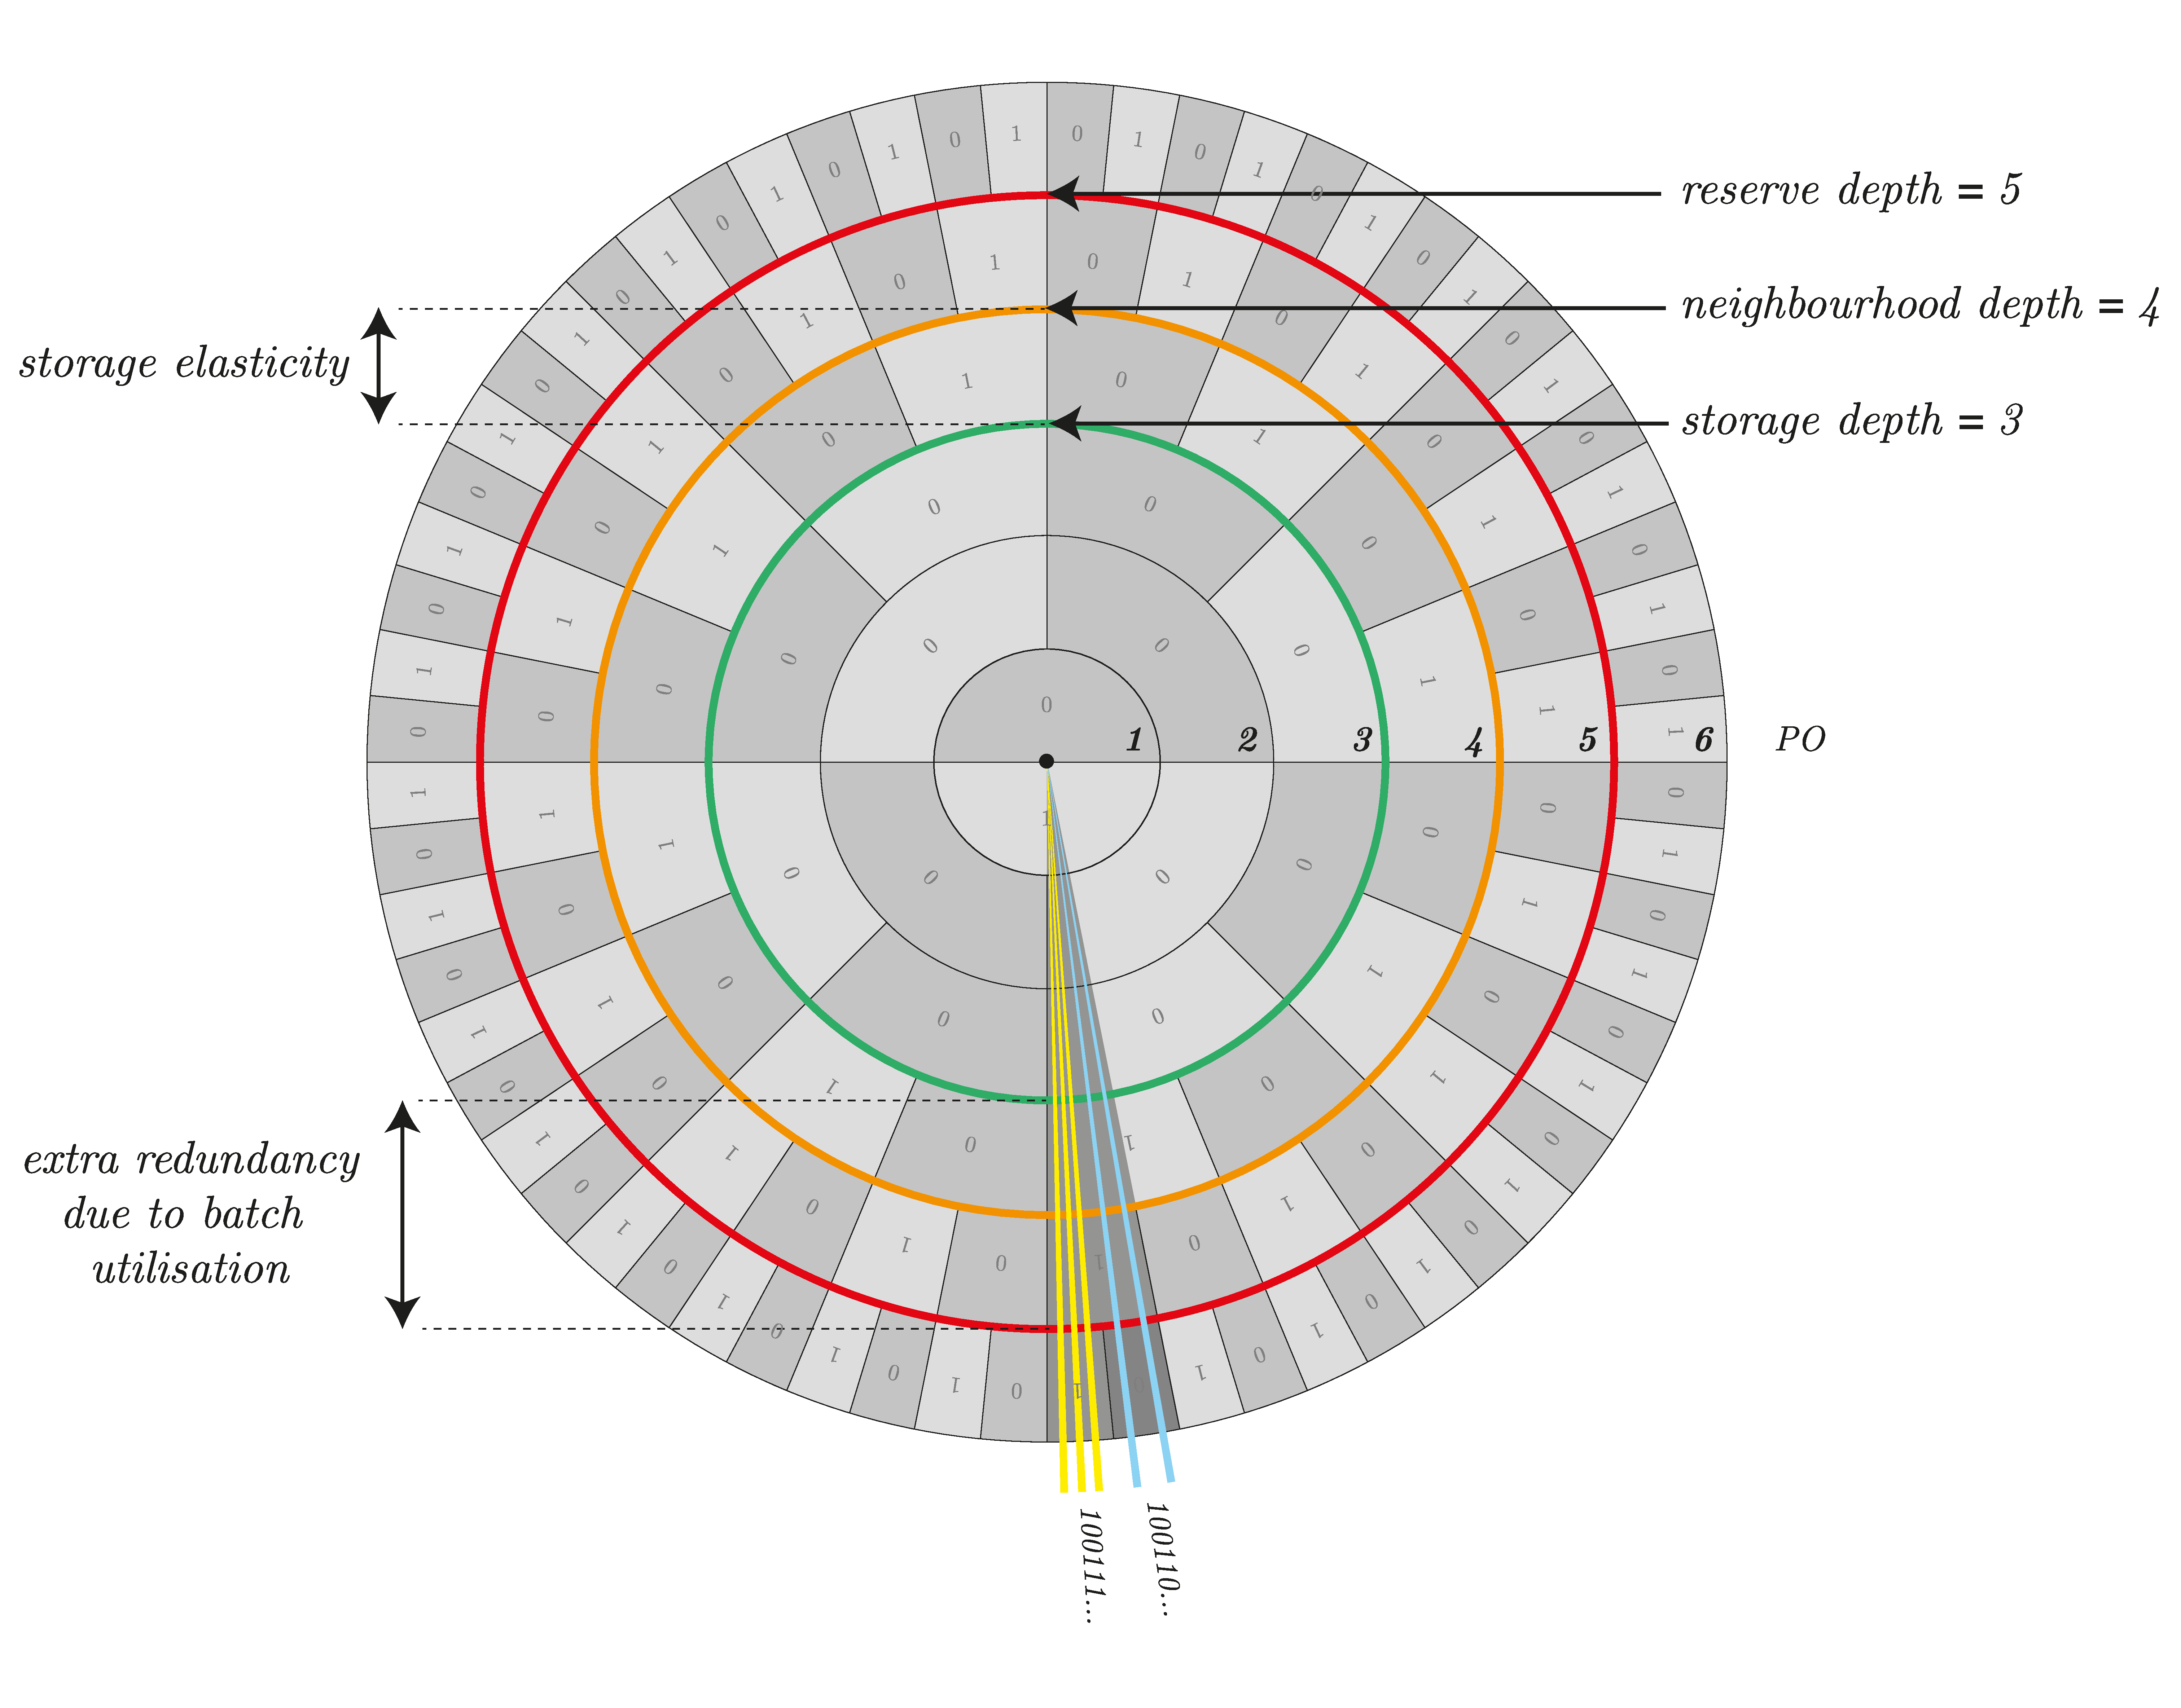
\includegraphics[width=.7\textwidth]{fig/depths-2.pdf}
  \caption[Depths]{The 3 depths (reserve, storage and neighbourhood) express the order of magnitude of reserved capacity (potential demand, red circle), uploaded chunks (effective demand, green circle) and the number of nodes (effective supply, orange circle), respectively. Their possible orderings express different scenarios with characteristic impact on data availability. Storage depth cannot be greater than reserve depth. A gap between storage depth and reserve depth quantifies the average batch utilisation rate. The gap between storage depth and a deeper neighbourhood depth quantifies the elasticity of the storage: the difference expresses how many times the effective volume can double before redundancy goes below required. While such oversupply may be anticipatory of growth in demand, if neighbourhood depth remains deeper than storage depth long term, it may indicate excessive profits. The opposite order indicates undersupply (redundancy below the desired level).}
\label{fig:depths}
\end{figure}    
%%%%%%%%%%%%%%%%%%%%%%%%%%%%%%%

% In the introduction we concluded that Swarm needs to have a subsystem for users to signal the importance/relevance of chunks. Postage stamps (and batches) were presented as a framework to implement storage incentives to ensure rarely accessed content remains available. 

%%%%%%%%%%%%%%%%%%%%%%%%%%%%%%%%%%%%%%%%%%%%%%%%%%%%%%%
\section{Fair redistribution}\label{sec:redistribution}


The system of positive%
%
\footnote{The concept of \emph{positive incentives} refers to a scheme whereby providers of a service are entitled to reward but there is no loss involved if they discontinue their service or are not online.}
%
storage incentives in Swarm is concerned with redistributing  to storage providers the BZZ tokens that uploaders deposited within the postage contract.%
%
\footnote{As explained earlier, uploaders pay in an unwithdrawable amount to the postage contract which serves as the balance to pay storage rent. In exchange they obtain the right to issue a fixed number of postage stamps which they attach to chunks they want the network to store.}
%
The overall balance on the contract covers the \gloss{reward pot} which represents the total \gloss{storage rent} cumulated over all postage batches for a particular period. The storage rent must be redistributed to storage providers in a way that guarantees that their earnings are proportional to their contribution weighing in storage space, quality of service and length of commitment.

The procedure for redistribution is best conceived of as a game orchestrated by a suite of smart contracts on the blockchain. Nodes earn the right to play through participation in storing and syncing chunks. 
The winners claim their reward by sending a transaction to the game contract. 

In section \ref{sec:uniformity-pot}, we formulate the idea of redistribution in terms of probabilistic outpayments to allow an easy proof of fairness. Next, in \ref{sec:mechanics}, we introduce the mechanics of the redistribution game.
Then, in \ref{sec:staking} and \ref{sec:por} we explain how we enforce maximum utilisation of dedicated storage for persisting  relevant content redundantly. We conclude in \ref{sec:price-oracle} by discussing how to read certain aspects of the game as price signals that render the network self-regulating through automatic price discovery. 

\subsection{Neighbourhoods, uniformity and probabilistic outpayments}\label{sec:uniformity-pot} 

In this section we argue that the efficient use of postage batches incentivises a balanced chunk distribution which in turn gives rise to uniform storage depth across neighbourhoods. We then explain how this enables a fair system of redistribution using probabilistic outpayments.
% \subsubsection{Uniformity}


Assuming an oracle that sets the unit price of storage, the storage rent due for a period of time for a batch can be calculated. The number of rent units for a batch is the result of multiplying the size of the batch with the number of blocks in the period. The price of rent is calculated from the number of rent units multiplied by the unit price.%
%
\footnote{If this theoretical amount is less than the the current balance of the batch, then the batch is expired and the effective rent is only the remaining balance.}
%
The total storage rent cumulated over all batches for the period between two outpayments constitutes the \emph{reward pot} for the round.

Instead of dividing the reward pot among neighbourhoods regularly, the entire reward pot can be transferred to (representative nodes in) one target neighbourhood in each round. This probabilistic outpayment scheme is fair on the level of neighbourhoods as long as we can make sure that over a large number of rounds the probability with which a  
neighbourhood is selected as the target corresponds to its relative contribution to the overall network storage. Given a constant prescribed reserve capacity and replication of the reserve content by nodes in a neighbourhood, each neighbourhood defined by storage depth contributes equally to the network. 

In section \ref{sec:postage-stamps}, we wrote that uploaders are strongly incentivised to use their postage batch in a way that the chunks they stamp with it are uniformly distributed across the address space. This being true of all batches creates a situation that chunks are uniformly distributed across the DISC. In particular, the sets of chunks sharing a prefix are expected to be roughly equal in size. Therefore we expect nodes to fill their prescribed reserve capacity with chunks at the same proximity order, irrespective of their location in the address space, i.e., the storage depth is uniform across  nodes and therefore across neighbourhoods.%
%
\footnote{Differences do occur due to variance but over many rounds, deviation from the mean is meant to be independent of the location.}
%
With neighbourhoods at equal depth, uniform sampling of neighbourhoods can be modelled by choosing the neighbourhood which contains an anchor (called the \emph{the neighbourhood selection anchor}%
%
% \footnote{one of the random nonces (see definition \ref{def:nonce-round}) from the \emph{random seed} of the round, see appendix \ref{sec:randomness}.}
%
) randomly dropped in the address space (see figure \ref{fig:neighbourhood-selection}).


\begin{figure}[!ht]
  \centering
    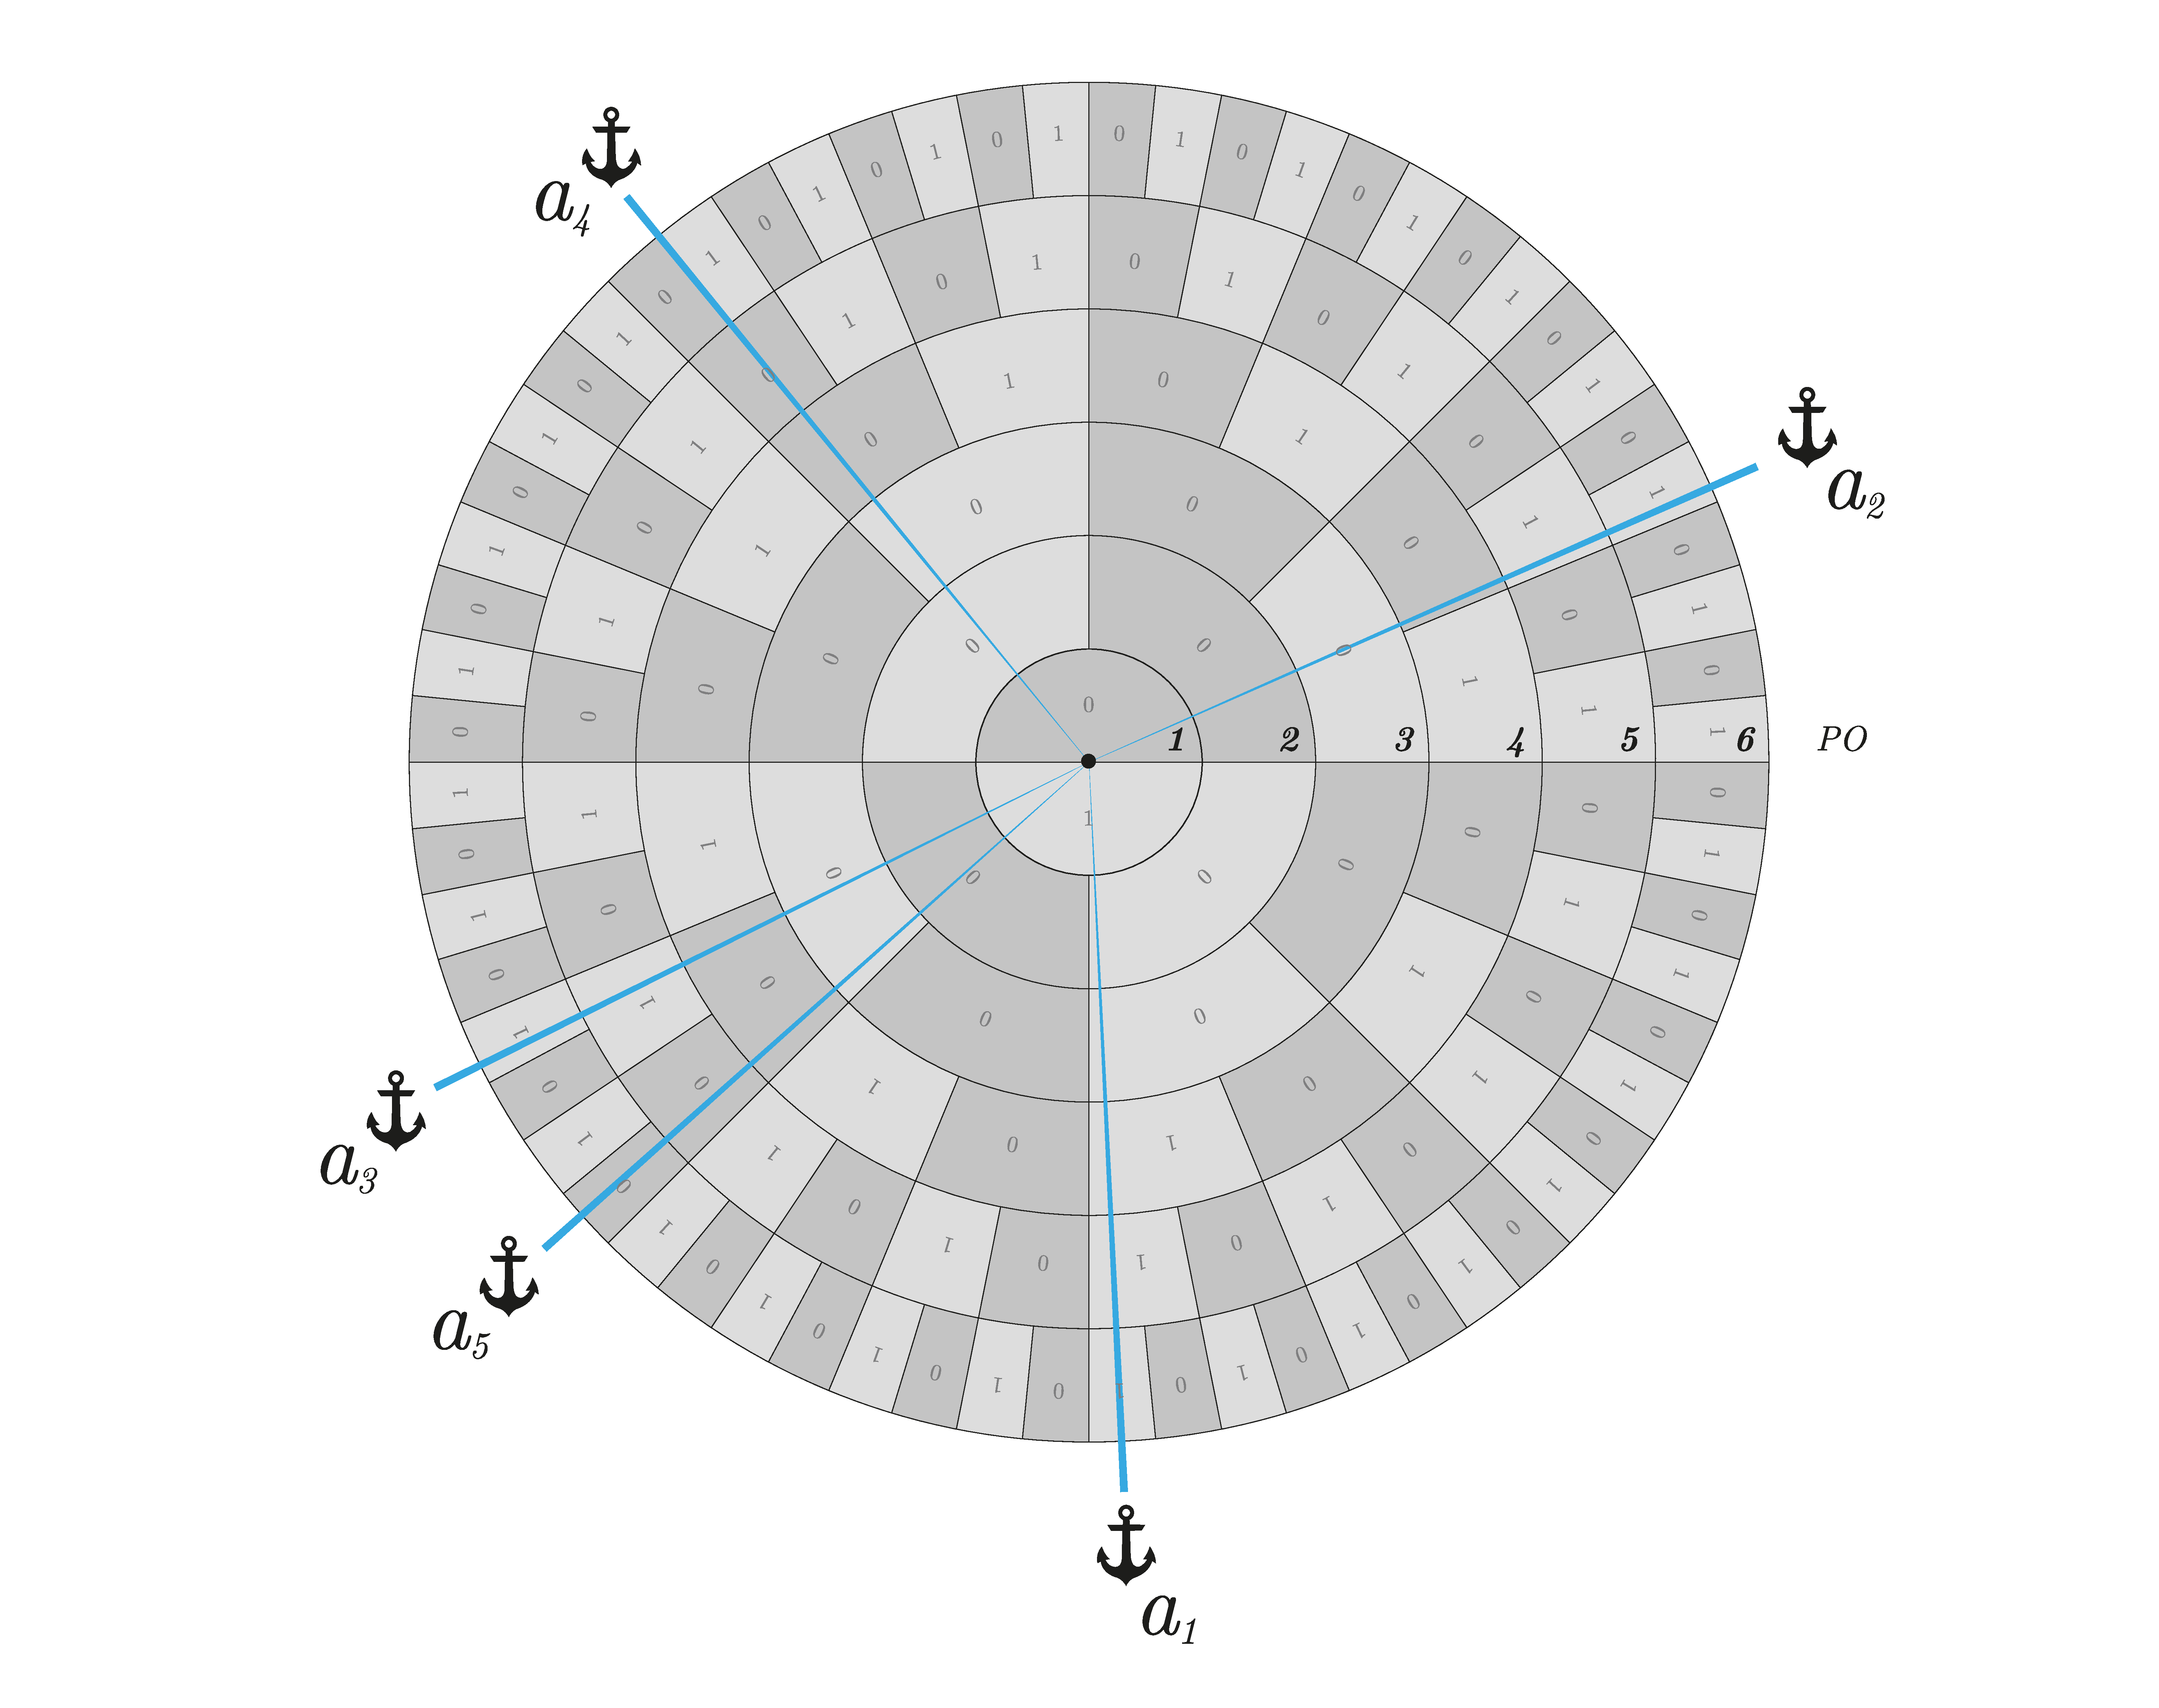
\includegraphics[width=\textwidth]{fig/nhd-selection.pdf}
  \caption[Neighbourhood selection and pot redistribution]{Neighbourhood selection and pot redistribution. The winning locality is selected by the neighbourhood selection anchor. Neighbourhoods that contain the anchor within their storage depth are invited to submit an application by committing to a consensual reserve sample. }
\label{fig:neighbourhood-selection}
\end{figure}    

    


\subsection{The mechanics of the redistribution game}\label{sec:mechanics}

The cooperation of peers to redundantly store for the network's benefit is underpinned by a \gloss{Schelling game}
% (defined formally in appendix \ref{sec:redistribution-game}) 
aimed at proving that the peers agree on the chunks they need to store and they do, in fact, store them. The redistribution game itself is orchestrated by the game contract, one of the building blocks of the system of 4 smart contracts which collectively drive the swarm storage incentive system (see figure \ref{fig:smart-contracts}):

\begin{itemize}
    \item[--] Postage contract -- serving as the batch store to sell postage batches to uploaders, keeping track of batch balances, batch expiry, storage rent and the reward pot itself.
    \item[--] Game contract -- orchestrates the redistribution rounds interacting with potential winners accepting commit, reveal and claim transactions from storage providers in selected neighbourhoods.
    \item[--] Staking contract -- operates a stake registry, maintaining committed stake and stake balance for nodes by their overlay; enables freezing and slashing of stake as well as withdrawal of surplus balance for stakers.
    \item[--] Price oracle -- maintains the unit price of  storage rent, accepts signals from the game contract to dynamically adjust according to supply and demand and provides current price oracle service for the other three contracts.
\end{itemize}


\begin{figure}[!ht]
  \centering
     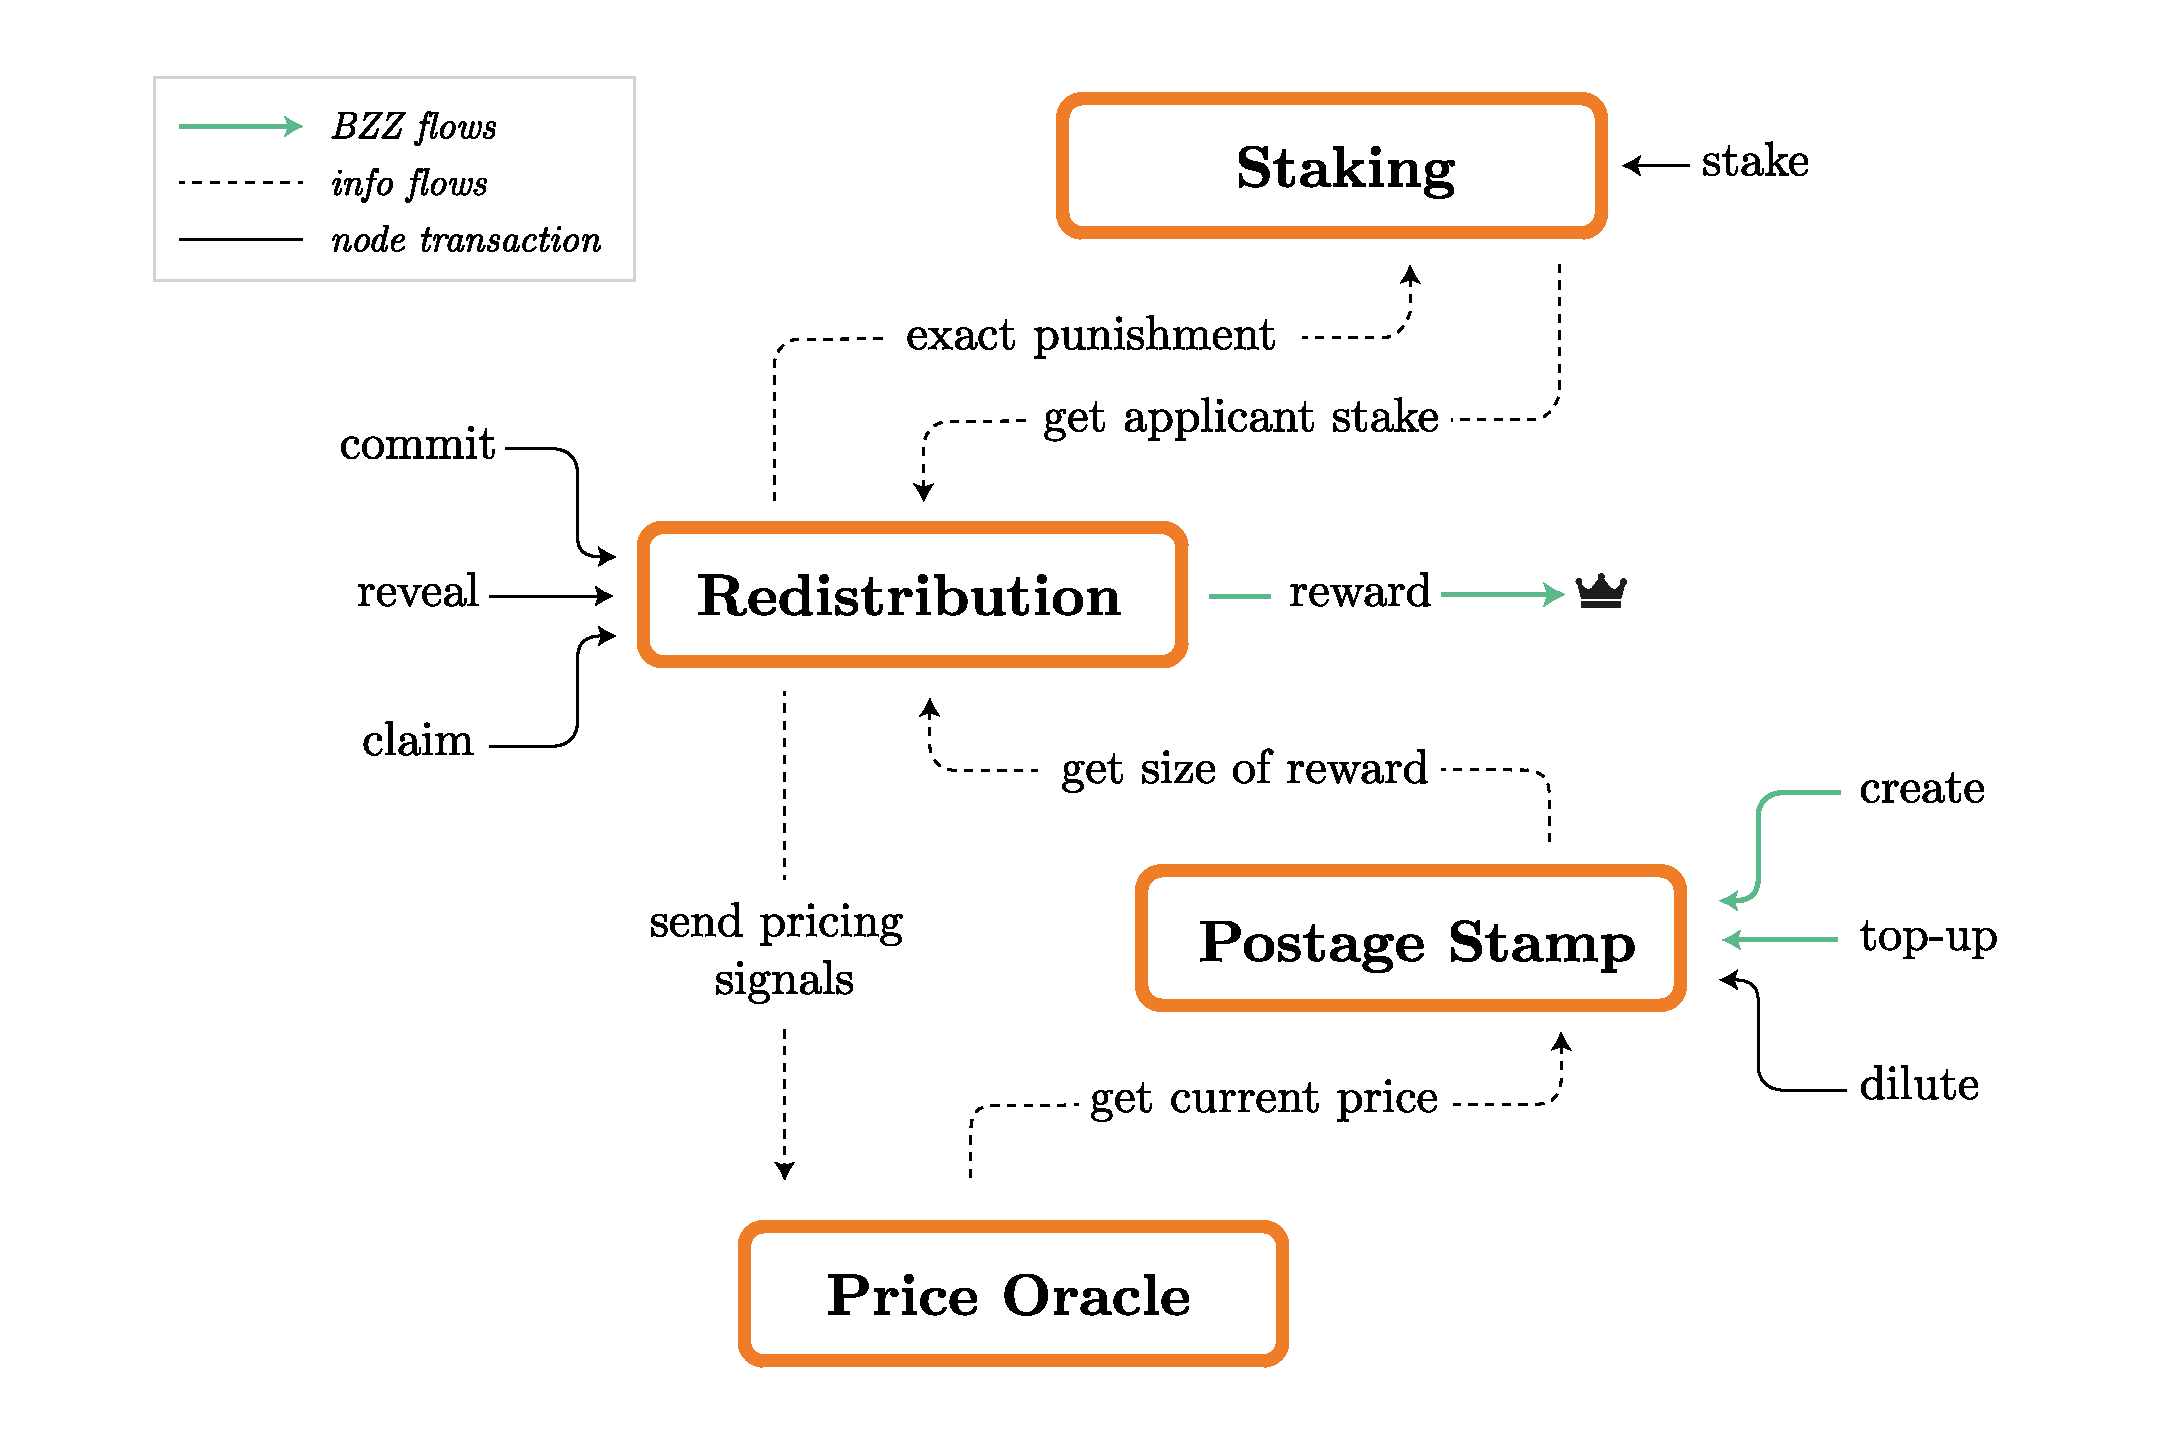
\includegraphics[width=\textwidth]{fig/smart-contract-interaction.pdf}
  \caption[Interaction of smart contracts for swarm storage incentives]{Interaction of smart contracts for swarm storage incentives. The figure shows with the dotted line the information flow between the four contracts comprising the storage incentive smart contract suite as well as the public transaction types they accept. }
\label{fig:smart-contracts}
\end{figure}    

The game is structured as a sequence of \emph{rounds}. Each round lasts for a fixed number of blocks and recur periodically. A round consists of 3 phases: \emph{commit}, \emph{reveal}, and \emph{claim}.%
%
\footnote{The commit and reveal phases are one quarter of the round length while the claim phase is one half.
}
%
The phases are named after the type of transaction the smart contract expects during that phase, and that nodes from the selected neighbourhood need to submit.%
%
\footnote{Both commit and reveal are simple and cheap transactions. The only expensive transaction is claim but that only the winner needs to submit.}
%
See figure \ref{fig:phases}

\begin{figure}[!ht]
  \centering
    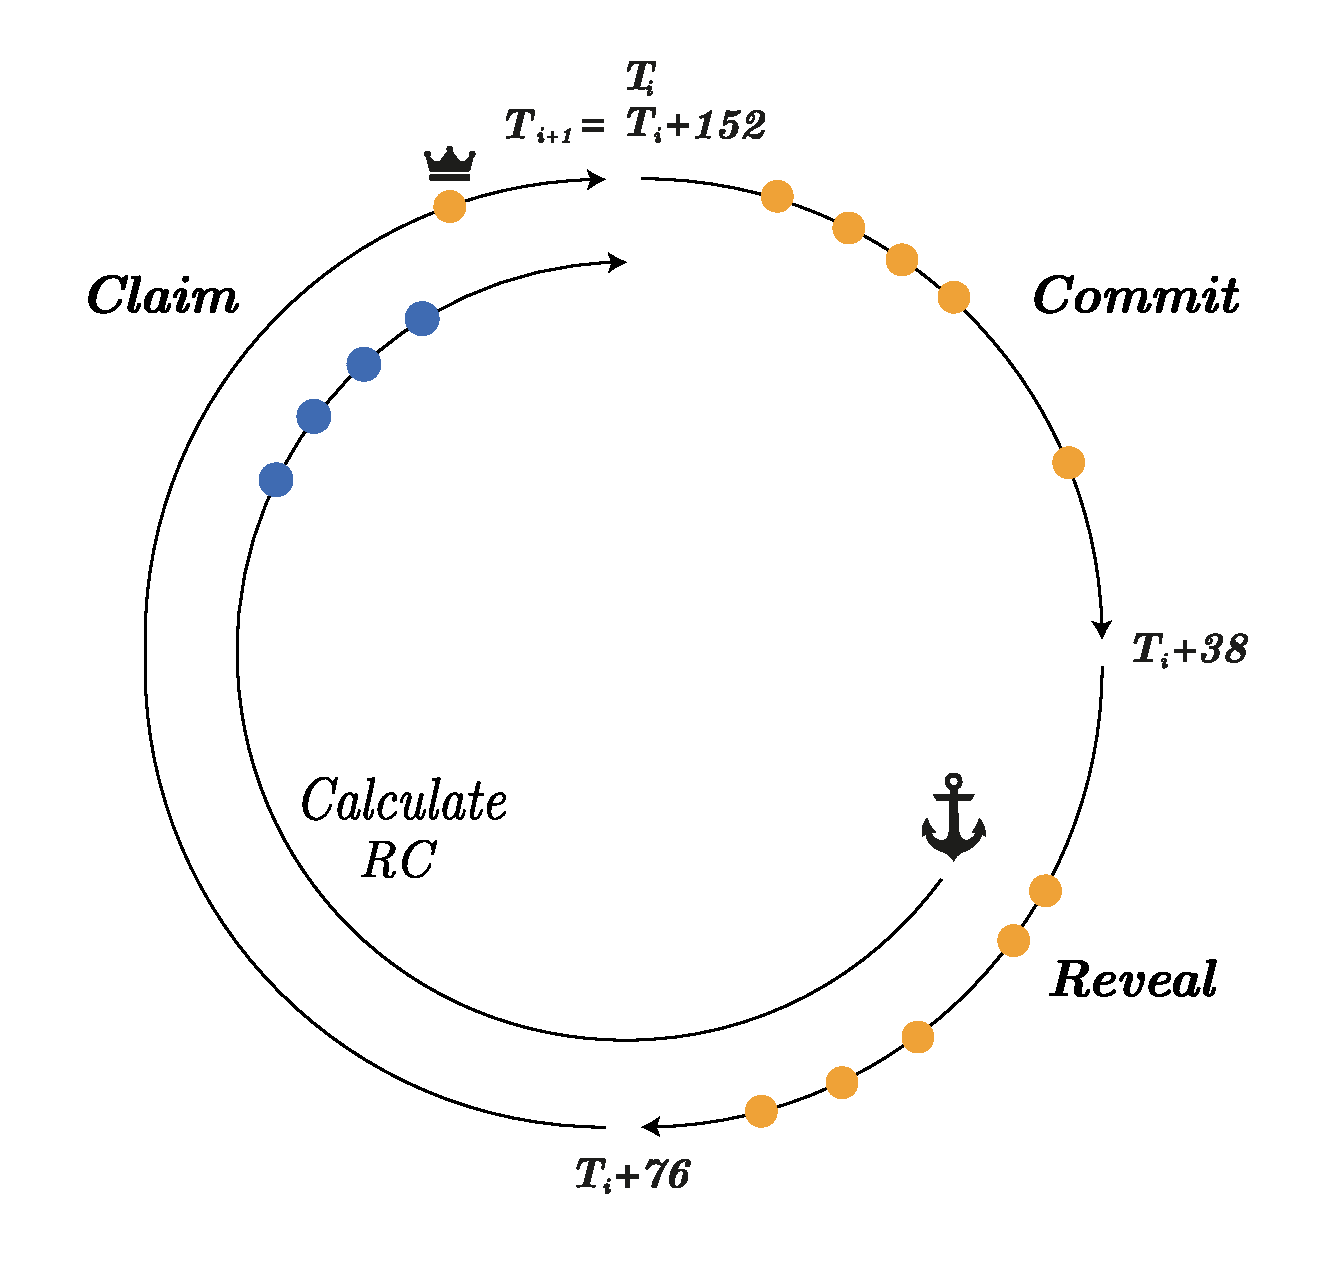
\includegraphics[width=.5\textwidth]{fig/round-lifecycle.pdf}
  \caption[Phases of a round of the redistribution game]{Phases of a round of the redistribution game. The figure displays the timeline of the repeating rounds of the redistribution game with its phases. In the context of smart contract interaction, logically starting with the commit phase, followed by reveal and claim. From the point of view of client node engagement starting with the end of the reveal phase with the neighbourhood selection anchor revealed, those in the selected neighbourhood start calculating their reserve sample only to submit it by the end of the next commit phase. If they are selected as an honest node and as a winner, they submit their proof of entitlement in a claim transaction.}
\label{fig:phases}
\end{figure}    

Once the reveal phase is over, the  \gloss{neighbourhood selection anchor} becomes known. Nodes that have the anchor within their neighbourhood%
%
\footnote{If storage depth is less than the anchor's proximity order relative to the overlay address.}
%
are  allowed to participate in the following round (see figure \ref{fig:neighbourhood-selection}).



The storer nodes in a neighbourhood are assumed to have  consensus over the chunks that make up their reserve and provide evidence called \gloss{proof of entitlement} to the blockchain (discussed below in detail in \ref{sec:por}). In such a game, the Nash-optimal strategy for each node is to follow the protocols and coordinate to guarantee that from the same information, all neighbouring peers will arrive at the same proof of entitlement. Since the proof of entitlement needs to be consensual but unstealable,%
%
\footnote{%
Any explicit communication between independent nodes about this reserve before the end of the commit phase constitutes risk in that it may leak the proof to a node not doing storage work. Therefore nodes are incentivised to keep the proof a secret. Making these proofs unstealable helps detect opportunistic peers that pose as storers but do not provide adequate storage.}
%
a commit/reveal scheme must be used.

In the \gloss{commit phase}, nodes in a neighbourhood will apply by submitting the \gloss{reserve commitment} obfuscated with an arbitrary key that they later reveal% 
% (see definition \ref{def:chc} in appendix \ref{sec:appendix-game})%
. The smart contract receiving the commit transaction verifies that the node is staked, i.e., the registry of the staking contract contains an entry for the node's overlay with a stake that is higher than the minimum stake.

In the \gloss{reveal phase}, each node that previously committed to a reserve, now reveal their commitment by submitting a transaction containing
their reserve commitments, their storage depth,
their overlay address, and the key they used to obfuscate  the commit.
When receiving the reveal transaction, the contract  verifies that the revealed data serialised does indeed hash to their commitment. It is also checked if the node belongs to the neighbourhood designated by the neighbourhood selection anchor, i.e., is within the storage depth provided in the reveal.

In the \gloss{claim phase}, the winner node must submit a claim transaction.%
%
\footnote{Every node in the selected neighbourhood needs to perform the corresponding calculations to determine whether or not they are the winner.}
%
First, in order to decide the outcome of the Schelling game, one reveal is selected  from among the reveals submitted during the reveal phase.%
%
\footnote{This is relevant only if the depth and/or the commitment are non-uniform across applicants.}
%
The selected reveal represents the truth; the set of applications agreeing with the selected one represent the \gloss{honest peers} of the neighbourhood, the ones disagreeing are the \gloss{liars}, while those committers that did not reveal or revealed invalid data are the \gloss{saboteurs}. Honesty is incentivised by the fact that liars and saboteurs get punished. In what follows we introduce staking that is needed for both the selection processes and the punitive measure.


\subsection{Staking}\label{sec:staking}

\subsubsection{Neighbours with shared storage}

In order to provide robust protection against accidental node churn, i.e., ensure retrievability of chunks from a neighbourhood in the face of some nodes being offline, the swarm require a number of independent storers in each neighbourhood physically replicating content.
If payout was given to each node that shows proof of entitlement, then operators would be incentivised to create spurious nodes with the sole purpose of applying for the reward. Measures can be introduced to enforce that these spurious nodes must be operating on the network, but ultimately, operators may choose to actually run several nodes yet share their storage on a single hardware. 
The incentive system must ensure that storage providers do not  adopt this strategy. To this end, we introduce \gloss{staking}.  

Stakes are used as weights by the contract to determine the true reserve commitment (truth selection) as well as the winner among the honest nodes (winner selection). Since peers' relative stake determine their chance of winning, stake is additive, i.e., operators' profit only depends on their total stake within the neighbourhood. Given the cost of running a node, operators will have no  motivation to divide their stake between multiple nodes sharing storage hardware.



\subsubsection{Committed stake and stake balance}

When registering in the staking contract, stakers commit to a stake denominated in rent units called 
\gloss{committed stake}.  The committed stake must have a lower bound.%
%
\footnote{A large number of staked nodes could cause the claim transaction to fail due to gas cost needed for iterating over them. This presents a potential attack where the adversary registers stakes for many nodes and commits for all of them. Such an attack is made prohibitively costly by enforcing a minimum stake.}
%
The  amount sent with the transaction is recorded and serves as collateral called \gloss{stake balance}. Stakes can be created or topped up any time, but the update time is recorded together with the amount.
Participation is restricted to peers whose stake has not changed recently, thereby excluding the possibility of changing stakes after knowing the selected neighbourhood.
Every time the stake of a node is queried, the contract returns  the  absolute committed stake in BZZ calculated as (1) the committed stake in rent units multiplied by the unit price of rent  or (2) the entire stake balance, whichever is smaller%
% (see definition \ref{def:stakes} in appendix \ref{sec:appendix-game})
.  

Stakes must be transferable between overlay addresses to facilitate neighbourhood hopping in case the distribution of stake per neighbourhood is unbalanced. 

\subsubsection{Withdrawability of surplus stake balance}



The committed stake lets operators express their  profit margin together with time preference for realising this profit. Since the profit is only transparent once the relative stakes within the neighbourhood are known, it is possible that nodes take a while to discover their optimal stake. 

If the BZZ token price increases and the unit price of rent drops, the entry for the node in the stake registry will show excess balance. This surplus can always be withdrawn,
and, as a consequence, stakers can realise their profit from BZZ appreciation.%
%
\footnote{In case the token price goes up substantially, the stake balance ends up worth much more than what nodes can ever expect to earn. If the stake balance was not at all withdrawable, participation would be disincentivised due to fear of losing the potential gains in the event of BZZ token appreciation.}
% 

 
%%%%%%%%%%%%%%%%%%%%%%%%%%%%%%%%%%%
\subsection{Neighbourhood consensus over the reserve}\label{sec:por}

Peers applying for the round must agree on which chunks belong to their respective reserves. For this, at the very least, the applicants must consent on their area of responsibility, which can be derived from their storage depth and their overlay address.  
The consensus over the reserve content is tested with the identity of a \gloss{reserve sample}.
The sample is the first $k$ chunks in the reserve using an ordering based on a modified hash of the chunks%
% (see \ref{def:transformed-reserve} in appendix \ref{sec:appendix-game})
.  The modified chunk hash is  obtained using the chunk contents and a \emph{salt} specific to the round.%
%
\footnote{This modified hash is the BMT hash of the chunk data using Keccak-256 prefixed with the reserve sample salt as a base hash%
% (defined in \ref{def:prefixed-hash} in appendix \ref{sec:appendix-game})
. The ordering is the ascending integer order reading the 32-byte modified hash as a big-endian encoded 256-bit integer%
% (see \ref{def:sampler} in appendix \ref{sec:appendix-game})
.}
%
It is impossible for any node to construct this set unless they store all (or a substantial number of the) valid chunks together with their data at or after the time the salt is revealed. 

\subsubsection{Recency and sampling}

The reserve sample must exclude too recent chunks because, otherwise, malicious uploaders could bombard nodes in the neighbourhood with a non-identical set of chunks  that are going to be sampled thereby breaking the consensus about the reserve. One way to guard against this attack is to save each chunk together with its time of storage%
%
\footnote{Using the timestamp within the postage stamp to define the minimum age on would not solve the consensus problem since chunks with old postage stamp could be circulated towards the end of sampling and cause disagreement between neighbours.}
% 
in the local database.
Pairwise synchronisation of chunks between neighbours with the pull-sync protocol respects this ordering by time of storage. 
We require that live syncing, i.e., syncing of chunks received after the peer connection started has a latency not longer than an agreed constant duration called \gloss{maximum syncing latency} (or \emph{max sync lag} for short). Peer connections lagging more with syncing are by protocol not counted as legit storer nodes. This restriction ensures that malicious nodes can not back-date new chunks more than the max sync lag without losing their storer status. 

In order to reach consensus, we must ensure that all chunks received by any node in the neighbourhood not later than $l$ should reach every node of the neighbourhood before the claim phase.
% This means that after receiving the chunk with a lag, the client still has time to include it in their sample and safely submit the commit transaction.
%
If we choose $l$ as 2 times the allowed sync lag then every chunk landing first with a node has time to arrive at each node to be safely included in a consensual sample.%
%
\footnote{Instead of actually monitoring neighbour connections and abstain from committing to a sample in case of excessive lag, one can just choose a small enough sample size.}%
%

\subsubsection{Storage depth and honest neighbourhood size}

In order to decide which reveal represents the truth for the current round, one submission out of all reveals is selected randomly with a probability proportional to the amount of stake the revealer has. More precisely: the amount of stake per neighbourhood size, i.e.,    \gloss{stake density}. The reserve sample hash and the reported storage depth thus revealed are considered the truth for the current round. 

Now we can understand why nodes will report actual storage depth correctly. If a node chooses to play with a larger neighbourhood than the neighbours, it will be selected more often than the others. However, as the committed storage depth decreases as compared to peers, the node's stake is counted with an exponentially deflated  value relative to the peers reporting a deeper storage radius, making such an attack costly.  

Overreporting storage depth is possible as long as the the node falls into this narrower proximity of the neighbourhood selection anchor. Therefore, a systematic exploit requires the malicious actor to control a staked node in each subneighbourhood of the true honest neighbourhood. 
On top of this, the winners also need to show evidence that the set of chunks within their storage depth do fill their reserve. 
The actual integer values of the transformed chunk addresses in the sample hold information regarding the size of the original sampled set.  
Requiring the size of the sampled set to fall within the expected range (with sufficient certainty) translates to imposing a constraint on the upper bound of the values of the sample. This construct is called \gloss{proof of density}% 
% (see definition \ref{def:chunk-density-validition} and appendix \ref{sec:density})%
.
%

Note that the sample-based density proof can be spoofed if the attacker is mining content filtering chunks in such a way that the transformed chunk addresses form a dense enough sample, then uses its own postage batches to stamp them. 
Further hardening against such attacks can be achieved by requiring  additionally a commitment to the entire set of postage stamps and similarly proving from a randomised sample the custody of a sufficient quantity. Due to this requirement, fraudulent claimants must not only generate the content, but must also have enough storage slots to fake the sample. This would require the attacker to purchase postage batches in the magnitude of the entire network 
or keep track of and store the actual postage stamps existing in the network. The former imposes a prohibitive cost on the attacker, whereas, in the latter case, the malicious claimant must bear the risk of relying on honest  neighbours for the post-hoc retrieval of witness chunk data needed for the proof of entitlement.
% See figure \ref{fig:proof-of-density}

% \begin{figure}[!ht]
%   \centering
%     % \includegraphics[width=\textwidth]{fig/rproof-of-density.pdf}
%   \caption[Proof of density]{Proof of density.}
% \label{fig:proof-of-density}
% \end{figure}    


\subsubsection{Skipped rounds and rollover}

If there is no claim in a given round, the pot simply rolls over and increase the outpayment for the next round of the redistribution. This policy is by far the easiest to implement, resulting in the lowest gas expenditures.% 
%
\footnote{One might argue for reimbursing honest nodes for their transaction costs. Thereby,  nodes with really small stakes can still participate and in general nodes are less exposed to variance in the probabilistic outpayments.}

\subsubsection{The eight rules of entitlement}

Here we summarise the eight rules of validating a claim (with committing and revealing a reserve commitment and then submitted evidence as proof of entitlement; see also table~\ref{tab:gr8}):%
%
% \footnote{The first three criteria are part of the conditions for staking, committing, and revealing (see definitions \ref{def:chc} and \ref{def:chs} for replication, \ref{def:stakes} and \ref{def:commits} for redundancy, \ref{def:reveals} for responsibility in appendix \ref{sec:appendix-game}. Relevance, retention, recency and  retrievability are proved as part of the proof of reserve (definition \ref{def:por}) and validated as part of the claim (\ref{def:por-validation}). Finally, proof of resources involves density proofs for chunks and stamps (definitions \ref{def:chc} and \ref{def:chs}) validated as part of the claim (definitions \ref{def:chunk-density-validition} and \ref{def:stamp-density-validition}, respectively). The specific construct of proof of entitlement is defined in \ref{def:poe} and its validation in \ref{def:claim-validation} in appendix \ref{sec:appendix-game}).}
%
\begin{itemize}[noitemsep]
%
\item[\hbox to 2em{\textsc{replication}}] \hspace{1cm}\\ Since liars get frozen (i.e., nodes that had revealed reserve commitment hash or storage depth different  from the winner are excluded from the game for a period), nodes in a neighbourhood are incentivised to replicate their reserve by syncronising the chunks they store using the pull-sync protocol.
%
\item[\hbox to 2em{\textsc{redundancy}}] \hspace{1cm}\\ The stake is used as weights in determining the within-neighbourhood probability of a node being selected as winner%
% (see \ref{def:winner-selection})%
. This implies no benefit in submitting multiple claims. Operators running multiple nodes in one neighbourhood (sharing storage) therefore have no advantage over running a single node with the same total stake. Assuming this disincentive to proliferate is effective, staking can be regarded as guarantee for true redundancy.
%
\item[\hbox to 2em{\textsc{responsibility}}] \hspace{1cm}\\  At the time of revealing it is checked if the neighbourhood selection anchor falls within the node's radius of responsibility, i.e., belong to the covered range of addresses whose proximity to the node's overlay address is not less than their reported storage depth. 
%
\item[\hbox to 2em{\textsc{relevance}}] \hspace{1cm}\\ Using a witness proof with the reserve commitment hash as root, we show evidence that an arbitrarily chosen segment in the reserve sample packed address chunk is the address of a witness chunk. 
A valid postage stamp signed off on this witness chunk address is presented to show that storing that chunk  in the reserve is relevant to someone (and is paid for). 
\item[\hbox to 2em{\textsc{retention}}] \hspace{1cm}\\ A segment inclusion proof is provided as evidence that the chunk data has been retained in full integrity. 
\item[\hbox to 2em{\textsc{recency}}] \hspace{1cm}\\ The salt used for the transformed reserve sample is derived from the current round's random nonce proving that the RS must have been compiled recently. The witness and segment indexes are derived from the next game's random seed ensuring that at the time of compilation and commitment, no compressed or partial retention of chunk data would have been
sufficient.
\item[\hbox to 2em{\textsc{retrievability}}] \hspace{1cm}\\  The chunk is shown to be retrievable by proximity based routing, i.e. its address belongs to the range of addresses covered by the neighbourhood: the chunk's proximity order to the node's overlay address is not less than their reported storage depth. 
\item[\hbox to 2em{\textsc{resources}}] \hspace{1cm}\\ Resource retention checks the volume of resources constituting the reserve by estimating the sampled set size via chunks density and stamps density. 
\end{itemize}


{\small \begin{longtable}{l|p{.4\textwidth}|p{.4\textwidth}}
\toprule
 {proof of} & {construct used} & {attacks mitigated}\\\midrule
 \textsc{replication}& Shelling-game over reserve sample& non-syncing, laggy syncing\\
 \textsc{redundancy}& share of reward proportional to stake & shared storage, over-application\\
 \textsc{responsibility}& proximity to anchor & depth/neighbourhood misreporting \\
 \textsc{relevance}& scarcity of postage stamps & generated data \\
 \textsc{retention}& segment inclusion proof & non-storage, partial storage\\
 \textsc{recency}& round-specific salt for reserve sample & create proof once and forget data\\
 \textsc{retrievability}& proximity of chunk & depth over-reporting\\ 
 \textsc{resources}& density-based reserve size estimation & targeted chunk generation (mining) \\\bottomrule
  \caption[r8: proofs used as evidence for entitlement to reward]{r8: proofs used as evidence for entitlement to reward.}
\label{tab:gr8}
 \end{longtable}
 }


\subsection{Pricing and network dynamics}\label{sec:price-oracle}

In this section, we first put the redistribution scheme in the context of self-sustainability, and provide a simple solution for price discovery.

For Swarm to be a truly self-sustaining system, the unit price of storage rent must be set in a way that is responsive to demand and supply. Ideally, the price is automatically adjusted based on reliable signals resulting in dynamic self-regulation. The guiding insight here is that the information storer nodes provide when  they apply for the redistribution game, also serves as a price signal. In other words, the redistribution game serves as a decentralised price oracle.



\subsubsection{Splitting and merging of neighbourhoods}

The storage depth represents the proximity radius within which the neighbourhood's storer nodes keep all chunks with valid postage stamps and fill their reserve. 


If the volume of newly issued storage slots from recently purchased batches (\emph{ingress rate}\/) and the volume of expired storage slots (\emph{outgress rate}\/) balance out, the storage depth remains unchanged.
But see what happens  if the volume of  reserved chunks increase?
Now, since the client's reserve capacity is constant, after a while, nodes are able to fill up their capacity with chunks that are at most one proximity order closer to them than the farthest chunks were previously, i.e.,  their storage depth increases.
When the volume of reserved chunks doubles,  the storage depth increases by one.  

In order to store this excess data under the same redundancy constraints the network requires double the number of nodes. If all else is equal, double the network-wide reserve, double the postage revenue and therefore double the overall pot that gets redistributed. When neighbourhoods split as they are absorbing the new volume, they simultaneously release the chunks in the PO bin of their old depth, i.e., the chunks now stored by their \gloss{sister nodes}. 

Utilisation rate is an organic way to  introduce pressure against fully maxing out a node's reserve with critical content, and thereby enable early detection of capacity pressure. This provides  sufficient safety buffer for the triggered incentives to take effect. For instance,  if utilisation rate is $1/8$, the storage depth is up to 3 PO-s shallower than the reserve depth.%
%
\footnote{The narrative of this scenario is that uploaders with underutilised batches subsidise extra redundancy for everyone.}
%
Now the ingress can be really high and bring the reserve depth down to storage depth. When the tendency of a closing gap between the potential (reserved) and actual (observed) utilisation of the DISC is detected, any incentive change will have the buffer to take effect without target redundancy being threatened. 

% See figure \ref{fig:pricing-demand}.


% \begin{figure}[!th]
%   \centering
%     % \includegraphics[width=.5\textwidth]{fig/pricing-demand.pdf}
%   \caption[Batch utilisation rate as a price signal]{Batch utilisation rate as a price signal.}
% \label{fig:pricing-demand}
% \end{figure}


\subsubsection{Number of honest nodes as price signal}

Since the storage capacity is maxed out, the ratio of supply and demand is directly seen in the number of honest nodes playing the Schelling game. 

We assume that if nodes are staying in the network for a longer period, their doing so testifies to their profitability. For a stable swarm, neighbourhoods need only 4 (balanced) nodes within as neighbourhood. Assuming equal stake (or more precisely, assuming that relative stake equalises profitability of node operators) if there are $n$ nodes in a neighbourhood, their long term profit is equally shared, this amount is optimised if there are exactly four nodes ($n=4$). This number can be more, since opportunistic operators may start their nodes in a complete neighbourhood in anticipation of a neighbourhood split due to capacity demand. As these nodes stay in, the same long term winnings of the neighbourhood gets distributed among more nodes than optimal.
However, the fact that nodes tolerate this implies that the reward is too much (the price is too high), and the network can tolerate a decreasing price.

On the other hand, if the number of honest revealers is less than the neighbourhood redundancy requirement, it signals capacity shortage and therefore requires the storage rent to increase. 

% See figure \ref{fig:pricing-supply}.

% \begin{figure}[!th]
%   \centering
%     % \includegraphics[width=.5\textwidth]{fig/pricing-supply.pdf}
%   \caption[Price signal for supply of storage capacity] {Price signal for supply of storage capacity.}
% \label{fig:pricing-supply}
% \end{figure}


\subsubsection{Parameterisation of the price oracle}

The rule for updating the price from one round to the next is that the current price is multiplied by a value $m$ which depends on the number of honest revealers in the round%
% (formally defined in appendix \ref{sec:appendix-price-oracle})%
. Mathematically, $p_{t+1} = m p_t$, where $p_t$ is the price in round $t$ (and $p_{t+1}$ is then the price in the following round). We define the multiplier $m$ in terms of the number of honest revealers $r$ and a stability parameter $\sigma$ governing how quickly the price should increase or decrease, all other things equal. 

\begin{figure}[!ht]
  \centering
  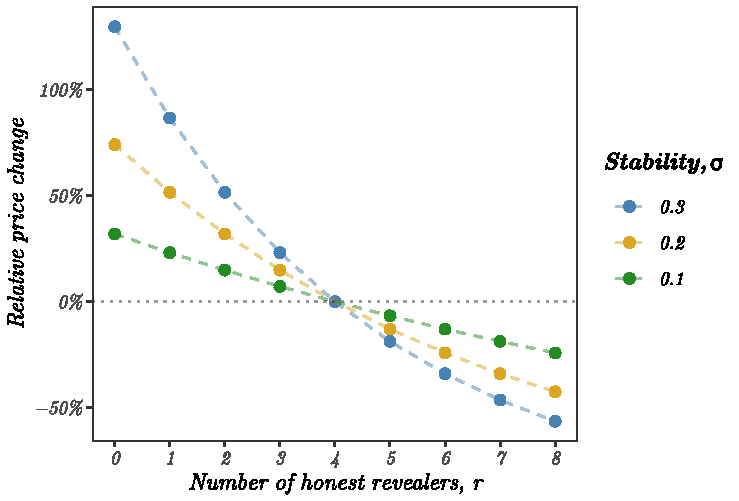
\includegraphics[width=.7\textwidth]{fig/adaptive-pricing.pdf}
  \caption[Adaptive pricing]{Adaptive pricing. The relative change in price (y-axis), mathematically expressed as the price in the next round divided by the price this round minus one ($p_{t+1} / p_t - 1$), is displayed against the number of honest revealers $r$ in the current round (x-axis). This is done so for three different values of the stability parameter $\sigma$ (colours). The points are the actual price change values; the connecting dashed lines are for visual aid only. The dotted horizontal line highlights the point at which no price change happens. Price change is exactly zero for any $\sigma$ when the number of honest revealers is four. Otherwise, larger values of $\sigma$ lead to larger relative price changes as the number of honest revealers is varied.}
  \label{fig:adaptive-pricing}
\end{figure}

In particular, we choose $m = 2^{\sigma(4 - r)}$, and therefore we have $p_{t+1} = 2^{\sigma(4 - r)} p_t$. This expresses how the deviation $4 - r$ of the number of revealers from the optimal value of 4 maps to an exponential change in price. The stability parameter $\sigma$ determines the generic smoothness of price changes across rounds, i.e., how many rounds it takes for the price of rent to double in case of a consistent signal of the lowest degree of undersupply (or halve in case of a consistent oversupply). Figure \ref{fig:adaptive-pricing} illustrates how the price model works.

Two minor adjustments are applied to this simple model. First, $r$ is capped at some value $r_{\text{max}}$ (chosen to be 8 in our case). That is, $r$ should actually be interpreted as the minimum of the number of honest revealers and $r_{\text{max}}$. Second, the price is never allowed to drop below some predetermined minimum $p_{\text{min}}$. That is, in case the price drop from one round to the next would bring the price below $p_{\text{min}}$, it will instead be kept at $p_{\text{min}}$. 

